\documentclass[twoside]{book}

% Packages required by doxygen
\usepackage{fixltx2e}
\usepackage{calc}
\usepackage{doxygen}
\usepackage[export]{adjustbox} % also loads graphicx
\usepackage{graphicx}
\usepackage[utf8]{inputenc}
\usepackage{makeidx}
\usepackage{multicol}
\usepackage{multirow}
\PassOptionsToPackage{warn}{textcomp}
\usepackage{textcomp}
\usepackage[nointegrals]{wasysym}
\usepackage[table]{xcolor}

% Font selection
\usepackage[T1]{fontenc}
\usepackage[scaled=.90]{helvet}
\usepackage{courier}
\usepackage{amssymb}
\usepackage{sectsty}
\renewcommand{\familydefault}{\sfdefault}
\allsectionsfont{%
  \fontseries{bc}\selectfont%
  \color{darkgray}%
}
\renewcommand{\DoxyLabelFont}{%
  \fontseries{bc}\selectfont%
  \color{darkgray}%
}
\newcommand{\+}{\discretionary{\mbox{\scriptsize$\hookleftarrow$}}{}{}}

% Page & text layout
\usepackage{geometry}
\geometry{%
  a4paper,%
  top=2.5cm,%
  bottom=2.5cm,%
  left=2.5cm,%
  right=2.5cm%
}
\tolerance=750
\hfuzz=15pt
\hbadness=750
\setlength{\emergencystretch}{15pt}
\setlength{\parindent}{0cm}
\setlength{\parskip}{3ex plus 2ex minus 2ex}
\makeatletter
\renewcommand{\paragraph}{%
  \@startsection{paragraph}{4}{0ex}{-1.0ex}{1.0ex}{%
    \normalfont\normalsize\bfseries\SS@parafont%
  }%
}
\renewcommand{\subparagraph}{%
  \@startsection{subparagraph}{5}{0ex}{-1.0ex}{1.0ex}{%
    \normalfont\normalsize\bfseries\SS@subparafont%
  }%
}
\makeatother

% Headers & footers
\usepackage{fancyhdr}
\pagestyle{fancyplain}
\fancyhead[LE]{\fancyplain{}{\bfseries\thepage}}
\fancyhead[CE]{\fancyplain{}{}}
\fancyhead[RE]{\fancyplain{}{\bfseries\leftmark}}
\fancyhead[LO]{\fancyplain{}{\bfseries\rightmark}}
\fancyhead[CO]{\fancyplain{}{}}
\fancyhead[RO]{\fancyplain{}{\bfseries\thepage}}
\fancyfoot[LE]{\fancyplain{}{}}
\fancyfoot[CE]{\fancyplain{}{}}
\fancyfoot[RE]{\fancyplain{}{\bfseries\scriptsize Generated by Doxygen }}
\fancyfoot[LO]{\fancyplain{}{\bfseries\scriptsize Generated by Doxygen }}
\fancyfoot[CO]{\fancyplain{}{}}
\fancyfoot[RO]{\fancyplain{}{}}
\renewcommand{\footrulewidth}{0.4pt}
\renewcommand{\chaptermark}[1]{%
  \markboth{#1}{}%
}
\renewcommand{\sectionmark}[1]{%
  \markright{\thesection\ #1}%
}

% Indices & bibliography
\usepackage{natbib}
\usepackage[titles]{tocloft}
\setcounter{tocdepth}{3}
\setcounter{secnumdepth}{5}
\makeindex

% Hyperlinks (required, but should be loaded last)
\usepackage{ifpdf}
\ifpdf
  \usepackage[pdftex,pagebackref=true]{hyperref}
\else
  \usepackage[ps2pdf,pagebackref=true]{hyperref}
\fi
\hypersetup{%
  colorlinks=true,%
  linkcolor=blue,%
  citecolor=blue,%
  unicode%
}

% Custom commands
\newcommand{\clearemptydoublepage}{%
  \newpage{\pagestyle{empty}\cleardoublepage}%
}

\usepackage{caption}
\captionsetup{labelsep=space,justification=centering,font={bf},singlelinecheck=off,skip=4pt,position=top}

%===== C O N T E N T S =====

\begin{document}

% Titlepage & ToC
\hypersetup{pageanchor=false,
             bookmarksnumbered=true,
             pdfencoding=unicode
            }
\pagenumbering{alph}
\begin{titlepage}
\vspace*{7cm}
\begin{center}%
{\Large munits }\\
\vspace*{1cm}
{\large Generated by Doxygen 1.8.13}\\
\end{center}
\end{titlepage}
\clearemptydoublepage
\pagenumbering{roman}
\tableofcontents
\clearemptydoublepage
\pagenumbering{arabic}
\hypersetup{pageanchor=true}

%--- Begin generated contents ---
\chapter{Namespace Index}
\section{Namespace List}
Here is a list of all namespaces with brief descriptions\+:\begin{DoxyCompactList}
\item\contentsline{section}{\hyperlink{namespacemunits}{munits} }{\pageref{namespacemunits}}{}
\end{DoxyCompactList}

\chapter{Hierarchical Index}
\section{Class Hierarchy}
This inheritance list is sorted roughly, but not completely, alphabetically\+:\begin{DoxyCompactList}
\item \contentsline{section}{munits\+:\+:Converter}{\pageref{classmunits_1_1_converter}}{}
\item \contentsline{section}{munits\+:\+:Converter\+Function}{\pageref{classmunits_1_1_converter_function}}{}
\begin{DoxyCompactList}
\item \contentsline{section}{munits\+:\+:Unit}{\pageref{classmunits_1_1_unit}}{}
\end{DoxyCompactList}
\item \contentsline{section}{munits\+:\+:Metric}{\pageref{structmunits_1_1_metric}}{}
\item \contentsline{section}{munits\+:\+:Prefix}{\pageref{classmunits_1_1_prefix}}{}
\item \contentsline{section}{munits\+:\+:Quantity}{\pageref{classmunits_1_1_quantity}}{}
\item \contentsline{section}{munits\+:\+:Resolver}{\pageref{classmunits_1_1_resolver}}{}
\item \contentsline{section}{munits\+:\+:Unit\+Notation}{\pageref{classmunits_1_1_unit_notation}}{}
\item \contentsline{section}{munits\+:\+:Unit\+Notation\+Vector}{\pageref{classmunits_1_1_unit_notation_vector}}{}
\end{DoxyCompactList}

\chapter{Class Index}
\section{Class List}
Here are the classes, structs, unions and interfaces with brief descriptions\+:\begin{DoxyCompactList}
\item\contentsline{section}{\hyperlink{classmunits_1_1_converter}{munits\+::\+Converter} }{\pageref{classmunits_1_1_converter}}{}
\item\contentsline{section}{\hyperlink{classmunits_1_1_converter_function}{munits\+::\+Converter\+Function} }{\pageref{classmunits_1_1_converter_function}}{}
\item\contentsline{section}{\hyperlink{structmunits_1_1_metric}{munits\+::\+Metric} }{\pageref{structmunits_1_1_metric}}{}
\item\contentsline{section}{\hyperlink{classmunits_1_1_prefix}{munits\+::\+Prefix} }{\pageref{classmunits_1_1_prefix}}{}
\item\contentsline{section}{\hyperlink{classmunits_1_1_quantity}{munits\+::\+Quantity} }{\pageref{classmunits_1_1_quantity}}{}
\item\contentsline{section}{\hyperlink{classmunits_1_1_resolver}{munits\+::\+Resolver} }{\pageref{classmunits_1_1_resolver}}{}
\item\contentsline{section}{\hyperlink{classmunits_1_1_unit}{munits\+::\+Unit} }{\pageref{classmunits_1_1_unit}}{}
\item\contentsline{section}{\hyperlink{classmunits_1_1_unit_notation}{munits\+::\+Unit\+Notation} }{\pageref{classmunits_1_1_unit_notation}}{}
\item\contentsline{section}{\hyperlink{classmunits_1_1_unit_notation_vector}{munits\+::\+Unit\+Notation\+Vector} }{\pageref{classmunits_1_1_unit_notation_vector}}{}
\end{DoxyCompactList}

\chapter{File Index}
\section{File List}
Here is a list of all files with brief descriptions\+:\begin{DoxyCompactList}
\item\contentsline{section}{Z\+:/ocs\+\_\+1/measurmentunits/src/\hyperlink{converter_8cpp}{converter.\+cpp} }{\pageref{converter_8cpp}}{}
\item\contentsline{section}{Z\+:/ocs\+\_\+1/measurmentunits/src/\hyperlink{converter_8hpp}{converter.\+hpp} }{\pageref{converter_8hpp}}{}
\item\contentsline{section}{Z\+:/ocs\+\_\+1/measurmentunits/src/\hyperlink{converter__function_8cpp}{converter\+\_\+function.\+cpp} }{\pageref{converter__function_8cpp}}{}
\item\contentsline{section}{Z\+:/ocs\+\_\+1/measurmentunits/src/\hyperlink{converter__function_8hpp}{converter\+\_\+function.\+hpp} }{\pageref{converter__function_8hpp}}{}
\item\contentsline{section}{Z\+:/ocs\+\_\+1/measurmentunits/src/\hyperlink{dynamic_8cpp}{dynamic.\+cpp} }{\pageref{dynamic_8cpp}}{}
\item\contentsline{section}{Z\+:/ocs\+\_\+1/measurmentunits/src/\hyperlink{dynamic_8hpp}{dynamic.\+hpp} }{\pageref{dynamic_8hpp}}{}
\item\contentsline{section}{Z\+:/ocs\+\_\+1/measurmentunits/src/\hyperlink{metric_8cpp}{metric.\+cpp} }{\pageref{metric_8cpp}}{}
\item\contentsline{section}{Z\+:/ocs\+\_\+1/measurmentunits/src/\hyperlink{metric_8hpp}{metric.\+hpp} }{\pageref{metric_8hpp}}{}
\item\contentsline{section}{Z\+:/ocs\+\_\+1/measurmentunits/src/\hyperlink{parsers_8cpp}{parsers.\+cpp} }{\pageref{parsers_8cpp}}{}
\item\contentsline{section}{Z\+:/ocs\+\_\+1/measurmentunits/src/\hyperlink{parsers_8hpp}{parsers.\+hpp} }{\pageref{parsers_8hpp}}{}
\item\contentsline{section}{Z\+:/ocs\+\_\+1/measurmentunits/src/\hyperlink{prefix_8cpp}{prefix.\+cpp} }{\pageref{prefix_8cpp}}{}
\item\contentsline{section}{Z\+:/ocs\+\_\+1/measurmentunits/src/\hyperlink{prefix_8hpp}{prefix.\+hpp} }{\pageref{prefix_8hpp}}{}
\item\contentsline{section}{Z\+:/ocs\+\_\+1/measurmentunits/src/\hyperlink{quantity_8cpp}{quantity.\+cpp} }{\pageref{quantity_8cpp}}{}
\item\contentsline{section}{Z\+:/ocs\+\_\+1/measurmentunits/src/\hyperlink{quantity_8h}{quantity.\+h} }{\pageref{quantity_8h}}{}
\item\contentsline{section}{Z\+:/ocs\+\_\+1/measurmentunits/src/\hyperlink{searchers_8cpp}{searchers.\+cpp} }{\pageref{searchers_8cpp}}{}
\item\contentsline{section}{Z\+:/ocs\+\_\+1/measurmentunits/src/\hyperlink{searchers_8hpp}{searchers.\+hpp} }{\pageref{searchers_8hpp}}{}
\item\contentsline{section}{Z\+:/ocs\+\_\+1/measurmentunits/src/\hyperlink{unit_8cpp}{unit.\+cpp} }{\pageref{unit_8cpp}}{}
\item\contentsline{section}{Z\+:/ocs\+\_\+1/measurmentunits/src/\hyperlink{unit_8hpp}{unit.\+hpp} }{\pageref{unit_8hpp}}{}
\item\contentsline{section}{Z\+:/ocs\+\_\+1/measurmentunits/src/\hyperlink{unit__notation_8cpp}{unit\+\_\+notation.\+cpp} }{\pageref{unit__notation_8cpp}}{}
\item\contentsline{section}{Z\+:/ocs\+\_\+1/measurmentunits/src/\hyperlink{unit__notation_8hpp}{unit\+\_\+notation.\+hpp} }{\pageref{unit__notation_8hpp}}{}
\item\contentsline{section}{Z\+:/ocs\+\_\+1/measurmentunits/src/\hyperlink{uresolver_8cpp}{uresolver.\+cpp} }{\pageref{uresolver_8cpp}}{}
\item\contentsline{section}{Z\+:/ocs\+\_\+1/measurmentunits/src/\hyperlink{uresolver_8hpp}{uresolver.\+hpp} }{\pageref{uresolver_8hpp}}{}
\end{DoxyCompactList}

\chapter{Namespace Documentation}
\hypertarget{namespacemunits}{}\section{munits Namespace Reference}
\label{namespacemunits}\index{munits@{munits}}
\subsection*{Classes}
\begin{DoxyCompactItemize}
\item 
class \hyperlink{classmunits_1_1_converter}{Converter}
\item 
class \hyperlink{classmunits_1_1_converter_function}{Converter\+Function}
\item 
struct \hyperlink{structmunits_1_1_metric}{Metric}
\item 
class \hyperlink{classmunits_1_1_prefix}{Prefix}
\item 
class \hyperlink{classmunits_1_1_quantity}{Quantity}
\item 
class \hyperlink{classmunits_1_1_resolver}{Resolver}
\item 
class \hyperlink{classmunits_1_1_unit}{Unit}
\item 
class \hyperlink{classmunits_1_1_unit_notation}{Unit\+Notation}
\item 
class \hyperlink{classmunits_1_1_unit_notation_vector}{Unit\+Notation\+Vector}
\end{DoxyCompactItemize}
\subsection*{Enumerations}
\begin{DoxyCompactItemize}
\item 
enum \hyperlink{namespacemunits_a22c8effe19fdc3eb888884aa217f0c25}{metrics} \{ \newline
\hyperlink{namespacemunits_a22c8effe19fdc3eb888884aa217f0c25af0df0f3284b638cfe6b62c61f8e946d9}{Length} = 0, 
\hyperlink{namespacemunits_a22c8effe19fdc3eb888884aa217f0c25ac8d62657f0c02eecd6df0021364f7ede}{Mass} = 1, 
\hyperlink{namespacemunits_a22c8effe19fdc3eb888884aa217f0c25a6c1dee69e2519642b5eebf9bd4cddc0a}{Time} = 2, 
\hyperlink{namespacemunits_a22c8effe19fdc3eb888884aa217f0c25a4bab5c7f1da3d1c44c296de66cdde6a3}{Electric\+Currency} = 3, 
\newline
\hyperlink{namespacemunits_a22c8effe19fdc3eb888884aa217f0c25aada9f930eb999d74dd9a465cf5ee0c87}{Temperature} = 4, 
\hyperlink{namespacemunits_a22c8effe19fdc3eb888884aa217f0c25af37da5a609a9a26c71c0efb86b2e7923}{Amount\+Of\+Substance} = 5, 
\hyperlink{namespacemunits_a22c8effe19fdc3eb888884aa217f0c25a902221490b14ba8a70f8de8f7aa325ff}{Luminous\+Intensity} = 6, 
\hyperlink{namespacemunits_a22c8effe19fdc3eb888884aa217f0c25ac0cf3600aa9c185366a4a009185f07e2}{Area} = 7, 
\newline
\hyperlink{namespacemunits_a22c8effe19fdc3eb888884aa217f0c25a7646730730e8c4359a1cc0f4e677aac2}{Volume} = 8, 
\hyperlink{namespacemunits_a22c8effe19fdc3eb888884aa217f0c25acb824d8937772e160e4e99344fd684e5}{Volumetric\+Flow} = 9, 
\hyperlink{namespacemunits_a22c8effe19fdc3eb888884aa217f0c25a95bf397f16724b9c09cf767f1a5370ae}{Molar\+Concentration} = 10, 
\hyperlink{namespacemunits_a22c8effe19fdc3eb888884aa217f0c25aa52f56fd97c134419e82eed2f6c0328e}{Acceleration} = 11, 
\newline
\hyperlink{namespacemunits_a22c8effe19fdc3eb888884aa217f0c25af54294b9cf0b439d7b10dba4a6dd090e}{Force} = 12, 
\hyperlink{namespacemunits_a22c8effe19fdc3eb888884aa217f0c25a39fb25786a08906bcc5bff1a59d6e49e}{Velocity} = 13, 
\hyperlink{namespacemunits_a22c8effe19fdc3eb888884aa217f0c25a0b9fb639baaabc426049ba1d672a33de}{Concentration} = 14, 
\hyperlink{namespacemunits_a22c8effe19fdc3eb888884aa217f0c25a5e05a5dc3174c342cac2884500674f26}{Density} = 14, 
\newline
\hyperlink{namespacemunits_a22c8effe19fdc3eb888884aa217f0c25a7c50a59d8b4745e14f11ce2f4635c39b}{Mass\+Flow} = 15, 
\hyperlink{namespacemunits_a22c8effe19fdc3eb888884aa217f0c25a69336d378661f6c003ce8bd521c6a585}{Pressure} = 16, 
\hyperlink{namespacemunits_a22c8effe19fdc3eb888884aa217f0c25afc27fb1897956e03e92c289bd07bc4e6}{Dynamic\+Viscosity} = 17, 
\hyperlink{namespacemunits_a22c8effe19fdc3eb888884aa217f0c25adfada9ac53008687de76e2b685c85e3f}{Kinematic\+Viscosity} = 18, 
\newline
\hyperlink{namespacemunits_a22c8effe19fdc3eb888884aa217f0c25aa8c947688502fa3bb484f7246334ea1c}{Power} = 19, 
\hyperlink{namespacemunits_a22c8effe19fdc3eb888884aa217f0c25a8ce48c97ce6a749f7c199dc6e6ca1e82}{Energy} = 20, 
\hyperlink{namespacemunits_a22c8effe19fdc3eb888884aa217f0c25ab39ca46fbd293fce76d4cdf7d329a7ad}{Voltage} = 21, 
\hyperlink{namespacemunits_a22c8effe19fdc3eb888884aa217f0c25ae58c92a28c016baaa26f6b43b19acb3a}{Frequency} = 22, 
\newline
\hyperlink{namespacemunits_a22c8effe19fdc3eb888884aa217f0c25a3dedc7ecc3ef28206254638a7a075763}{Electric\+Charge} = 23, 
\hyperlink{namespacemunits_a22c8effe19fdc3eb888884aa217f0c25aebe93335a2da9557293202acc6f107b2}{Electric\+Capacitance} = 24, 
\hyperlink{namespacemunits_a22c8effe19fdc3eb888884aa217f0c25abe6f3b22c1951e7fc2c74d25676b43c0}{Electric\+Resistance} = 25, 
\hyperlink{namespacemunits_a22c8effe19fdc3eb888884aa217f0c25a08eb24223a082d1e77c1065b5ecd941e}{Electrical\+Conductance} = 26, 
\newline
\hyperlink{namespacemunits_a22c8effe19fdc3eb888884aa217f0c25a403ee91a73605ae3906b530771a6c7a5}{Magnetic\+Flux} = 27, 
\hyperlink{namespacemunits_a22c8effe19fdc3eb888884aa217f0c25a46579a9b5189d4159bdbde3cf0b733a9}{Magnetic\+Flux\+Density} = 28, 
\hyperlink{namespacemunits_a22c8effe19fdc3eb888884aa217f0c25a586f648f184805d655f97b94421bdcee}{Inductance} = 29, 
\hyperlink{namespacemunits_a22c8effe19fdc3eb888884aa217f0c25a7fc37598d9c1e89b5b05d5423f040dec}{Illuminance} = 30, 
\newline
\hyperlink{namespacemunits_a22c8effe19fdc3eb888884aa217f0c25a0831ca7f466dbf14db10706ff0b25ab5}{Absorbed\+Dose} = 31, 
\hyperlink{namespacemunits_a22c8effe19fdc3eb888884aa217f0c25ab773206a8a5f7a622d5374913ba05ee1}{Catalytic\+Activity} = 32, 
\hyperlink{namespacemunits_a22c8effe19fdc3eb888884aa217f0c25aa304e63cc2c9c51d6dc50d42488a9476}{\+\_\+\+Last}
 \}
\end{DoxyCompactItemize}
\subsection*{Functions}
\begin{DoxyCompactItemize}
\item 
const std\+::vector$<$ \hyperlink{structmunits_1_1_metric}{munits\+::\+Metric} $>$ \& \hyperlink{namespacemunits_a8bf80780c6ef4ce5b588d266a2de306e}{Get\+Matrix} ()
\item 
const std\+::map$<$ std\+::string, const std\+::shared\+\_\+ptr$<$ \hyperlink{classmunits_1_1_converter_function}{Converter\+Function} $>$ $>$ \& \hyperlink{namespacemunits_a43150beff0a68af86df9d5a02e69b334}{Get\+Prefixes} ()
\item 
std\+::vector$<$ std\+::string $>$ \hyperlink{namespacemunits_a0035cd1272a835c8d06716a9e866b720}{unparser} (std\+::string unit)
\item 
std\+::vector$<$ std\+::string $>$ \hyperlink{namespacemunits_a10ce8183cbfa4ab0a239a45c56f4dcbe}{rparser} (std\+::string token)
\item 
\hyperlink{classmunits_1_1_quantity}{Quantity} \hyperlink{namespacemunits_a38a90819b6f9b539204ec66e73b60a93}{pow} (const \hyperlink{classmunits_1_1_quantity}{Quantity} \&a, int e)
\item 
const long long int \hyperlink{namespacemunits_a31a640e781f471e914e53e370cdf63ef}{get\+Matrix\+Index} (const std\+::vector$<$ int $>$ \&searched)
\item 
const double \hyperlink{namespacemunits_ad54c1c999ca5e614726f2204bca2b988}{get\+Exponent\+Of\+Prefix} (const std\+::string prefix)
\item 
const std\+::string \hyperlink{namespacemunits_a9ee8078d5f9db8759156a3ff38f9cf39}{get\+Prefix\+By\+Exponent} (int exponent)
\item 
const int \hyperlink{namespacemunits_a49bfbd8f3668a72e3d5404be4a4ee0df}{get\+Max\+Prefix\+Exponent} ()
\item 
const int \hyperlink{namespacemunits_a348f0717c758e64ada5ef3811299af38}{get\+Min\+Prefix\+Exponent} ()
\item 
const \hyperlink{namespacemunits_a22c8effe19fdc3eb888884aa217f0c25}{metrics} \hyperlink{namespacemunits_a252f17286e532b20b64968b1c7f80f7e}{get\+Metric} (const std\+::vector$<$ int $>$ \&searched)
\end{DoxyCompactItemize}


\subsection{Enumeration Type Documentation}
\mbox{\Hypertarget{namespacemunits_a22c8effe19fdc3eb888884aa217f0c25}\label{namespacemunits_a22c8effe19fdc3eb888884aa217f0c25}} 
\index{munits@{munits}!metrics@{metrics}}
\index{metrics@{metrics}!munits@{munits}}
\subsubsection{\texorpdfstring{metrics}{metrics}}
{\footnotesize\ttfamily enum \hyperlink{namespacemunits_a22c8effe19fdc3eb888884aa217f0c25}{munits\+::metrics}}

\begin{DoxyEnumFields}{Enumerator}
\raisebox{\heightof{T}}[0pt][0pt]{\index{Length@{Length}!munits@{munits}}\index{munits@{munits}!Length@{Length}}}\mbox{\Hypertarget{namespacemunits_a22c8effe19fdc3eb888884aa217f0c25af0df0f3284b638cfe6b62c61f8e946d9}\label{namespacemunits_a22c8effe19fdc3eb888884aa217f0c25af0df0f3284b638cfe6b62c61f8e946d9}} 
Length&\\
\hline

\raisebox{\heightof{T}}[0pt][0pt]{\index{Mass@{Mass}!munits@{munits}}\index{munits@{munits}!Mass@{Mass}}}\mbox{\Hypertarget{namespacemunits_a22c8effe19fdc3eb888884aa217f0c25ac8d62657f0c02eecd6df0021364f7ede}\label{namespacemunits_a22c8effe19fdc3eb888884aa217f0c25ac8d62657f0c02eecd6df0021364f7ede}} 
Mass&\\
\hline

\raisebox{\heightof{T}}[0pt][0pt]{\index{Time@{Time}!munits@{munits}}\index{munits@{munits}!Time@{Time}}}\mbox{\Hypertarget{namespacemunits_a22c8effe19fdc3eb888884aa217f0c25a6c1dee69e2519642b5eebf9bd4cddc0a}\label{namespacemunits_a22c8effe19fdc3eb888884aa217f0c25a6c1dee69e2519642b5eebf9bd4cddc0a}} 
Time&\\
\hline

\raisebox{\heightof{T}}[0pt][0pt]{\index{Electric\+Currency@{Electric\+Currency}!munits@{munits}}\index{munits@{munits}!Electric\+Currency@{Electric\+Currency}}}\mbox{\Hypertarget{namespacemunits_a22c8effe19fdc3eb888884aa217f0c25a4bab5c7f1da3d1c44c296de66cdde6a3}\label{namespacemunits_a22c8effe19fdc3eb888884aa217f0c25a4bab5c7f1da3d1c44c296de66cdde6a3}} 
Electric\+Currency&\\
\hline

\raisebox{\heightof{T}}[0pt][0pt]{\index{Temperature@{Temperature}!munits@{munits}}\index{munits@{munits}!Temperature@{Temperature}}}\mbox{\Hypertarget{namespacemunits_a22c8effe19fdc3eb888884aa217f0c25aada9f930eb999d74dd9a465cf5ee0c87}\label{namespacemunits_a22c8effe19fdc3eb888884aa217f0c25aada9f930eb999d74dd9a465cf5ee0c87}} 
Temperature&\\
\hline

\raisebox{\heightof{T}}[0pt][0pt]{\index{Amount\+Of\+Substance@{Amount\+Of\+Substance}!munits@{munits}}\index{munits@{munits}!Amount\+Of\+Substance@{Amount\+Of\+Substance}}}\mbox{\Hypertarget{namespacemunits_a22c8effe19fdc3eb888884aa217f0c25af37da5a609a9a26c71c0efb86b2e7923}\label{namespacemunits_a22c8effe19fdc3eb888884aa217f0c25af37da5a609a9a26c71c0efb86b2e7923}} 
Amount\+Of\+Substance&\\
\hline

\raisebox{\heightof{T}}[0pt][0pt]{\index{Luminous\+Intensity@{Luminous\+Intensity}!munits@{munits}}\index{munits@{munits}!Luminous\+Intensity@{Luminous\+Intensity}}}\mbox{\Hypertarget{namespacemunits_a22c8effe19fdc3eb888884aa217f0c25a902221490b14ba8a70f8de8f7aa325ff}\label{namespacemunits_a22c8effe19fdc3eb888884aa217f0c25a902221490b14ba8a70f8de8f7aa325ff}} 
Luminous\+Intensity&\\
\hline

\raisebox{\heightof{T}}[0pt][0pt]{\index{Area@{Area}!munits@{munits}}\index{munits@{munits}!Area@{Area}}}\mbox{\Hypertarget{namespacemunits_a22c8effe19fdc3eb888884aa217f0c25ac0cf3600aa9c185366a4a009185f07e2}\label{namespacemunits_a22c8effe19fdc3eb888884aa217f0c25ac0cf3600aa9c185366a4a009185f07e2}} 
Area&\\
\hline

\raisebox{\heightof{T}}[0pt][0pt]{\index{Volume@{Volume}!munits@{munits}}\index{munits@{munits}!Volume@{Volume}}}\mbox{\Hypertarget{namespacemunits_a22c8effe19fdc3eb888884aa217f0c25a7646730730e8c4359a1cc0f4e677aac2}\label{namespacemunits_a22c8effe19fdc3eb888884aa217f0c25a7646730730e8c4359a1cc0f4e677aac2}} 
Volume&\\
\hline

\raisebox{\heightof{T}}[0pt][0pt]{\index{Volumetric\+Flow@{Volumetric\+Flow}!munits@{munits}}\index{munits@{munits}!Volumetric\+Flow@{Volumetric\+Flow}}}\mbox{\Hypertarget{namespacemunits_a22c8effe19fdc3eb888884aa217f0c25acb824d8937772e160e4e99344fd684e5}\label{namespacemunits_a22c8effe19fdc3eb888884aa217f0c25acb824d8937772e160e4e99344fd684e5}} 
Volumetric\+Flow&\\
\hline

\raisebox{\heightof{T}}[0pt][0pt]{\index{Molar\+Concentration@{Molar\+Concentration}!munits@{munits}}\index{munits@{munits}!Molar\+Concentration@{Molar\+Concentration}}}\mbox{\Hypertarget{namespacemunits_a22c8effe19fdc3eb888884aa217f0c25a95bf397f16724b9c09cf767f1a5370ae}\label{namespacemunits_a22c8effe19fdc3eb888884aa217f0c25a95bf397f16724b9c09cf767f1a5370ae}} 
Molar\+Concentration&\\
\hline

\raisebox{\heightof{T}}[0pt][0pt]{\index{Acceleration@{Acceleration}!munits@{munits}}\index{munits@{munits}!Acceleration@{Acceleration}}}\mbox{\Hypertarget{namespacemunits_a22c8effe19fdc3eb888884aa217f0c25aa52f56fd97c134419e82eed2f6c0328e}\label{namespacemunits_a22c8effe19fdc3eb888884aa217f0c25aa52f56fd97c134419e82eed2f6c0328e}} 
Acceleration&\\
\hline

\raisebox{\heightof{T}}[0pt][0pt]{\index{Force@{Force}!munits@{munits}}\index{munits@{munits}!Force@{Force}}}\mbox{\Hypertarget{namespacemunits_a22c8effe19fdc3eb888884aa217f0c25af54294b9cf0b439d7b10dba4a6dd090e}\label{namespacemunits_a22c8effe19fdc3eb888884aa217f0c25af54294b9cf0b439d7b10dba4a6dd090e}} 
Force&\\
\hline

\raisebox{\heightof{T}}[0pt][0pt]{\index{Velocity@{Velocity}!munits@{munits}}\index{munits@{munits}!Velocity@{Velocity}}}\mbox{\Hypertarget{namespacemunits_a22c8effe19fdc3eb888884aa217f0c25a39fb25786a08906bcc5bff1a59d6e49e}\label{namespacemunits_a22c8effe19fdc3eb888884aa217f0c25a39fb25786a08906bcc5bff1a59d6e49e}} 
Velocity&\\
\hline

\raisebox{\heightof{T}}[0pt][0pt]{\index{Concentration@{Concentration}!munits@{munits}}\index{munits@{munits}!Concentration@{Concentration}}}\mbox{\Hypertarget{namespacemunits_a22c8effe19fdc3eb888884aa217f0c25a0b9fb639baaabc426049ba1d672a33de}\label{namespacemunits_a22c8effe19fdc3eb888884aa217f0c25a0b9fb639baaabc426049ba1d672a33de}} 
Concentration&\\
\hline

\raisebox{\heightof{T}}[0pt][0pt]{\index{Density@{Density}!munits@{munits}}\index{munits@{munits}!Density@{Density}}}\mbox{\Hypertarget{namespacemunits_a22c8effe19fdc3eb888884aa217f0c25a5e05a5dc3174c342cac2884500674f26}\label{namespacemunits_a22c8effe19fdc3eb888884aa217f0c25a5e05a5dc3174c342cac2884500674f26}} 
Density&\\
\hline

\raisebox{\heightof{T}}[0pt][0pt]{\index{Mass\+Flow@{Mass\+Flow}!munits@{munits}}\index{munits@{munits}!Mass\+Flow@{Mass\+Flow}}}\mbox{\Hypertarget{namespacemunits_a22c8effe19fdc3eb888884aa217f0c25a7c50a59d8b4745e14f11ce2f4635c39b}\label{namespacemunits_a22c8effe19fdc3eb888884aa217f0c25a7c50a59d8b4745e14f11ce2f4635c39b}} 
Mass\+Flow&\\
\hline

\raisebox{\heightof{T}}[0pt][0pt]{\index{Pressure@{Pressure}!munits@{munits}}\index{munits@{munits}!Pressure@{Pressure}}}\mbox{\Hypertarget{namespacemunits_a22c8effe19fdc3eb888884aa217f0c25a69336d378661f6c003ce8bd521c6a585}\label{namespacemunits_a22c8effe19fdc3eb888884aa217f0c25a69336d378661f6c003ce8bd521c6a585}} 
Pressure&\\
\hline

\raisebox{\heightof{T}}[0pt][0pt]{\index{Dynamic\+Viscosity@{Dynamic\+Viscosity}!munits@{munits}}\index{munits@{munits}!Dynamic\+Viscosity@{Dynamic\+Viscosity}}}\mbox{\Hypertarget{namespacemunits_a22c8effe19fdc3eb888884aa217f0c25afc27fb1897956e03e92c289bd07bc4e6}\label{namespacemunits_a22c8effe19fdc3eb888884aa217f0c25afc27fb1897956e03e92c289bd07bc4e6}} 
Dynamic\+Viscosity&\\
\hline

\raisebox{\heightof{T}}[0pt][0pt]{\index{Kinematic\+Viscosity@{Kinematic\+Viscosity}!munits@{munits}}\index{munits@{munits}!Kinematic\+Viscosity@{Kinematic\+Viscosity}}}\mbox{\Hypertarget{namespacemunits_a22c8effe19fdc3eb888884aa217f0c25adfada9ac53008687de76e2b685c85e3f}\label{namespacemunits_a22c8effe19fdc3eb888884aa217f0c25adfada9ac53008687de76e2b685c85e3f}} 
Kinematic\+Viscosity&\\
\hline

\raisebox{\heightof{T}}[0pt][0pt]{\index{Power@{Power}!munits@{munits}}\index{munits@{munits}!Power@{Power}}}\mbox{\Hypertarget{namespacemunits_a22c8effe19fdc3eb888884aa217f0c25aa8c947688502fa3bb484f7246334ea1c}\label{namespacemunits_a22c8effe19fdc3eb888884aa217f0c25aa8c947688502fa3bb484f7246334ea1c}} 
Power&\\
\hline

\raisebox{\heightof{T}}[0pt][0pt]{\index{Energy@{Energy}!munits@{munits}}\index{munits@{munits}!Energy@{Energy}}}\mbox{\Hypertarget{namespacemunits_a22c8effe19fdc3eb888884aa217f0c25a8ce48c97ce6a749f7c199dc6e6ca1e82}\label{namespacemunits_a22c8effe19fdc3eb888884aa217f0c25a8ce48c97ce6a749f7c199dc6e6ca1e82}} 
Energy&\\
\hline

\raisebox{\heightof{T}}[0pt][0pt]{\index{Voltage@{Voltage}!munits@{munits}}\index{munits@{munits}!Voltage@{Voltage}}}\mbox{\Hypertarget{namespacemunits_a22c8effe19fdc3eb888884aa217f0c25ab39ca46fbd293fce76d4cdf7d329a7ad}\label{namespacemunits_a22c8effe19fdc3eb888884aa217f0c25ab39ca46fbd293fce76d4cdf7d329a7ad}} 
Voltage&\\
\hline

\raisebox{\heightof{T}}[0pt][0pt]{\index{Frequency@{Frequency}!munits@{munits}}\index{munits@{munits}!Frequency@{Frequency}}}\mbox{\Hypertarget{namespacemunits_a22c8effe19fdc3eb888884aa217f0c25ae58c92a28c016baaa26f6b43b19acb3a}\label{namespacemunits_a22c8effe19fdc3eb888884aa217f0c25ae58c92a28c016baaa26f6b43b19acb3a}} 
Frequency&\\
\hline

\raisebox{\heightof{T}}[0pt][0pt]{\index{Electric\+Charge@{Electric\+Charge}!munits@{munits}}\index{munits@{munits}!Electric\+Charge@{Electric\+Charge}}}\mbox{\Hypertarget{namespacemunits_a22c8effe19fdc3eb888884aa217f0c25a3dedc7ecc3ef28206254638a7a075763}\label{namespacemunits_a22c8effe19fdc3eb888884aa217f0c25a3dedc7ecc3ef28206254638a7a075763}} 
Electric\+Charge&\\
\hline

\raisebox{\heightof{T}}[0pt][0pt]{\index{Electric\+Capacitance@{Electric\+Capacitance}!munits@{munits}}\index{munits@{munits}!Electric\+Capacitance@{Electric\+Capacitance}}}\mbox{\Hypertarget{namespacemunits_a22c8effe19fdc3eb888884aa217f0c25aebe93335a2da9557293202acc6f107b2}\label{namespacemunits_a22c8effe19fdc3eb888884aa217f0c25aebe93335a2da9557293202acc6f107b2}} 
Electric\+Capacitance&\\
\hline

\raisebox{\heightof{T}}[0pt][0pt]{\index{Electric\+Resistance@{Electric\+Resistance}!munits@{munits}}\index{munits@{munits}!Electric\+Resistance@{Electric\+Resistance}}}\mbox{\Hypertarget{namespacemunits_a22c8effe19fdc3eb888884aa217f0c25abe6f3b22c1951e7fc2c74d25676b43c0}\label{namespacemunits_a22c8effe19fdc3eb888884aa217f0c25abe6f3b22c1951e7fc2c74d25676b43c0}} 
Electric\+Resistance&\\
\hline

\raisebox{\heightof{T}}[0pt][0pt]{\index{Electrical\+Conductance@{Electrical\+Conductance}!munits@{munits}}\index{munits@{munits}!Electrical\+Conductance@{Electrical\+Conductance}}}\mbox{\Hypertarget{namespacemunits_a22c8effe19fdc3eb888884aa217f0c25a08eb24223a082d1e77c1065b5ecd941e}\label{namespacemunits_a22c8effe19fdc3eb888884aa217f0c25a08eb24223a082d1e77c1065b5ecd941e}} 
Electrical\+Conductance&\\
\hline

\raisebox{\heightof{T}}[0pt][0pt]{\index{Magnetic\+Flux@{Magnetic\+Flux}!munits@{munits}}\index{munits@{munits}!Magnetic\+Flux@{Magnetic\+Flux}}}\mbox{\Hypertarget{namespacemunits_a22c8effe19fdc3eb888884aa217f0c25a403ee91a73605ae3906b530771a6c7a5}\label{namespacemunits_a22c8effe19fdc3eb888884aa217f0c25a403ee91a73605ae3906b530771a6c7a5}} 
Magnetic\+Flux&\\
\hline

\raisebox{\heightof{T}}[0pt][0pt]{\index{Magnetic\+Flux\+Density@{Magnetic\+Flux\+Density}!munits@{munits}}\index{munits@{munits}!Magnetic\+Flux\+Density@{Magnetic\+Flux\+Density}}}\mbox{\Hypertarget{namespacemunits_a22c8effe19fdc3eb888884aa217f0c25a46579a9b5189d4159bdbde3cf0b733a9}\label{namespacemunits_a22c8effe19fdc3eb888884aa217f0c25a46579a9b5189d4159bdbde3cf0b733a9}} 
Magnetic\+Flux\+Density&\\
\hline

\raisebox{\heightof{T}}[0pt][0pt]{\index{Inductance@{Inductance}!munits@{munits}}\index{munits@{munits}!Inductance@{Inductance}}}\mbox{\Hypertarget{namespacemunits_a22c8effe19fdc3eb888884aa217f0c25a586f648f184805d655f97b94421bdcee}\label{namespacemunits_a22c8effe19fdc3eb888884aa217f0c25a586f648f184805d655f97b94421bdcee}} 
Inductance&\\
\hline

\raisebox{\heightof{T}}[0pt][0pt]{\index{Illuminance@{Illuminance}!munits@{munits}}\index{munits@{munits}!Illuminance@{Illuminance}}}\mbox{\Hypertarget{namespacemunits_a22c8effe19fdc3eb888884aa217f0c25a7fc37598d9c1e89b5b05d5423f040dec}\label{namespacemunits_a22c8effe19fdc3eb888884aa217f0c25a7fc37598d9c1e89b5b05d5423f040dec}} 
Illuminance&\\
\hline

\raisebox{\heightof{T}}[0pt][0pt]{\index{Absorbed\+Dose@{Absorbed\+Dose}!munits@{munits}}\index{munits@{munits}!Absorbed\+Dose@{Absorbed\+Dose}}}\mbox{\Hypertarget{namespacemunits_a22c8effe19fdc3eb888884aa217f0c25a0831ca7f466dbf14db10706ff0b25ab5}\label{namespacemunits_a22c8effe19fdc3eb888884aa217f0c25a0831ca7f466dbf14db10706ff0b25ab5}} 
Absorbed\+Dose&\\
\hline

\raisebox{\heightof{T}}[0pt][0pt]{\index{Catalytic\+Activity@{Catalytic\+Activity}!munits@{munits}}\index{munits@{munits}!Catalytic\+Activity@{Catalytic\+Activity}}}\mbox{\Hypertarget{namespacemunits_a22c8effe19fdc3eb888884aa217f0c25ab773206a8a5f7a622d5374913ba05ee1}\label{namespacemunits_a22c8effe19fdc3eb888884aa217f0c25ab773206a8a5f7a622d5374913ba05ee1}} 
Catalytic\+Activity&\\
\hline

\raisebox{\heightof{T}}[0pt][0pt]{\index{\+\_\+\+Last@{\+\_\+\+Last}!munits@{munits}}\index{munits@{munits}!\+\_\+\+Last@{\+\_\+\+Last}}}\mbox{\Hypertarget{namespacemunits_a22c8effe19fdc3eb888884aa217f0c25aa304e63cc2c9c51d6dc50d42488a9476}\label{namespacemunits_a22c8effe19fdc3eb888884aa217f0c25aa304e63cc2c9c51d6dc50d42488a9476}} 
\+\_\+\+Last&\\
\hline

\end{DoxyEnumFields}


\subsection{Function Documentation}
\mbox{\Hypertarget{namespacemunits_ad54c1c999ca5e614726f2204bca2b988}\label{namespacemunits_ad54c1c999ca5e614726f2204bca2b988}} 
\index{munits@{munits}!get\+Exponent\+Of\+Prefix@{get\+Exponent\+Of\+Prefix}}
\index{get\+Exponent\+Of\+Prefix@{get\+Exponent\+Of\+Prefix}!munits@{munits}}
\subsubsection{\texorpdfstring{get\+Exponent\+Of\+Prefix()}{getExponentOfPrefix()}}
{\footnotesize\ttfamily const double munits\+::get\+Exponent\+Of\+Prefix (\begin{DoxyParamCaption}\item[{const std\+::string}]{prefix }\end{DoxyParamCaption})}

\mbox{\Hypertarget{namespacemunits_a8bf80780c6ef4ce5b588d266a2de306e}\label{namespacemunits_a8bf80780c6ef4ce5b588d266a2de306e}} 
\index{munits@{munits}!Get\+Matrix@{Get\+Matrix}}
\index{Get\+Matrix@{Get\+Matrix}!munits@{munits}}
\subsubsection{\texorpdfstring{Get\+Matrix()}{GetMatrix()}}
{\footnotesize\ttfamily const std\+::vector$<$ \hyperlink{structmunits_1_1_metric}{munits\+::\+Metric} $>$ \& munits\+::\+Get\+Matrix (\begin{DoxyParamCaption}{ }\end{DoxyParamCaption})}

\mbox{\Hypertarget{namespacemunits_a31a640e781f471e914e53e370cdf63ef}\label{namespacemunits_a31a640e781f471e914e53e370cdf63ef}} 
\index{munits@{munits}!get\+Matrix\+Index@{get\+Matrix\+Index}}
\index{get\+Matrix\+Index@{get\+Matrix\+Index}!munits@{munits}}
\subsubsection{\texorpdfstring{get\+Matrix\+Index()}{getMatrixIndex()}}
{\footnotesize\ttfamily const long long int munits\+::get\+Matrix\+Index (\begin{DoxyParamCaption}\item[{const std\+::vector$<$ int $>$ \&}]{searched }\end{DoxyParamCaption})}

\mbox{\Hypertarget{namespacemunits_a49bfbd8f3668a72e3d5404be4a4ee0df}\label{namespacemunits_a49bfbd8f3668a72e3d5404be4a4ee0df}} 
\index{munits@{munits}!get\+Max\+Prefix\+Exponent@{get\+Max\+Prefix\+Exponent}}
\index{get\+Max\+Prefix\+Exponent@{get\+Max\+Prefix\+Exponent}!munits@{munits}}
\subsubsection{\texorpdfstring{get\+Max\+Prefix\+Exponent()}{getMaxPrefixExponent()}}
{\footnotesize\ttfamily const int munits\+::get\+Max\+Prefix\+Exponent (\begin{DoxyParamCaption}{ }\end{DoxyParamCaption})}

\mbox{\Hypertarget{namespacemunits_a252f17286e532b20b64968b1c7f80f7e}\label{namespacemunits_a252f17286e532b20b64968b1c7f80f7e}} 
\index{munits@{munits}!get\+Metric@{get\+Metric}}
\index{get\+Metric@{get\+Metric}!munits@{munits}}
\subsubsection{\texorpdfstring{get\+Metric()}{getMetric()}}
{\footnotesize\ttfamily const \hyperlink{namespacemunits_a22c8effe19fdc3eb888884aa217f0c25}{munits\+::metrics} munits\+::get\+Metric (\begin{DoxyParamCaption}\item[{const std\+::vector$<$ int $>$ \&}]{searched }\end{DoxyParamCaption})}

\mbox{\Hypertarget{namespacemunits_a348f0717c758e64ada5ef3811299af38}\label{namespacemunits_a348f0717c758e64ada5ef3811299af38}} 
\index{munits@{munits}!get\+Min\+Prefix\+Exponent@{get\+Min\+Prefix\+Exponent}}
\index{get\+Min\+Prefix\+Exponent@{get\+Min\+Prefix\+Exponent}!munits@{munits}}
\subsubsection{\texorpdfstring{get\+Min\+Prefix\+Exponent()}{getMinPrefixExponent()}}
{\footnotesize\ttfamily const int munits\+::get\+Min\+Prefix\+Exponent (\begin{DoxyParamCaption}{ }\end{DoxyParamCaption})}

\mbox{\Hypertarget{namespacemunits_a9ee8078d5f9db8759156a3ff38f9cf39}\label{namespacemunits_a9ee8078d5f9db8759156a3ff38f9cf39}} 
\index{munits@{munits}!get\+Prefix\+By\+Exponent@{get\+Prefix\+By\+Exponent}}
\index{get\+Prefix\+By\+Exponent@{get\+Prefix\+By\+Exponent}!munits@{munits}}
\subsubsection{\texorpdfstring{get\+Prefix\+By\+Exponent()}{getPrefixByExponent()}}
{\footnotesize\ttfamily const std\+::string munits\+::get\+Prefix\+By\+Exponent (\begin{DoxyParamCaption}\item[{int}]{exponent }\end{DoxyParamCaption})}

\mbox{\Hypertarget{namespacemunits_a43150beff0a68af86df9d5a02e69b334}\label{namespacemunits_a43150beff0a68af86df9d5a02e69b334}} 
\index{munits@{munits}!Get\+Prefixes@{Get\+Prefixes}}
\index{Get\+Prefixes@{Get\+Prefixes}!munits@{munits}}
\subsubsection{\texorpdfstring{Get\+Prefixes()}{GetPrefixes()}}
{\footnotesize\ttfamily const std\+::map$<$ std\+::string, const std\+::shared\+\_\+ptr$<$ \hyperlink{classmunits_1_1_converter_function}{munits\+::\+Converter\+Function} $>$ $>$ \& munits\+::\+Get\+Prefixes (\begin{DoxyParamCaption}{ }\end{DoxyParamCaption})}

\mbox{\Hypertarget{namespacemunits_a38a90819b6f9b539204ec66e73b60a93}\label{namespacemunits_a38a90819b6f9b539204ec66e73b60a93}} 
\index{munits@{munits}!pow@{pow}}
\index{pow@{pow}!munits@{munits}}
\subsubsection{\texorpdfstring{pow()}{pow()}}
{\footnotesize\ttfamily \hyperlink{classmunits_1_1_quantity}{munits\+::\+Quantity} munits\+::pow (\begin{DoxyParamCaption}\item[{const \hyperlink{classmunits_1_1_quantity}{Quantity} \&}]{a,  }\item[{int}]{e }\end{DoxyParamCaption})}

\mbox{\Hypertarget{namespacemunits_a10ce8183cbfa4ab0a239a45c56f4dcbe}\label{namespacemunits_a10ce8183cbfa4ab0a239a45c56f4dcbe}} 
\index{munits@{munits}!rparser@{rparser}}
\index{rparser@{rparser}!munits@{munits}}
\subsubsection{\texorpdfstring{rparser()}{rparser()}}
{\footnotesize\ttfamily std\+::vector$<$std\+::string$>$ munits\+::rparser (\begin{DoxyParamCaption}\item[{std\+::string}]{token }\end{DoxyParamCaption})}

\mbox{\Hypertarget{namespacemunits_a0035cd1272a835c8d06716a9e866b720}\label{namespacemunits_a0035cd1272a835c8d06716a9e866b720}} 
\index{munits@{munits}!unparser@{unparser}}
\index{unparser@{unparser}!munits@{munits}}
\subsubsection{\texorpdfstring{unparser()}{unparser()}}
{\footnotesize\ttfamily std\+::vector$<$std\+::string$>$ munits\+::unparser (\begin{DoxyParamCaption}\item[{std\+::string}]{unit }\end{DoxyParamCaption})}


\chapter{Class Documentation}
\hypertarget{classmunits_1_1_converter}{}\section{munits\+:\+:Converter Class Reference}
\label{classmunits_1_1_converter}\index{munits\+::\+Converter@{munits\+::\+Converter}}


{\ttfamily \#include $<$converter.\+hpp$>$}

\subsection*{Public Member Functions}
\begin{DoxyCompactItemize}
\item 
const std\+::map$<$ std\+::string, const std\+::shared\+\_\+ptr$<$ \hyperlink{classmunits_1_1_converter_function}{Converter\+Function} $>$ $>$ \& \hyperlink{classmunits_1_1_converter_a48a8ab27724c3aa86e9f36bc8699ae22}{Prefixes} () const
\item 
const std\+::map$<$ std\+::string, const std\+::shared\+\_\+ptr$<$ \hyperlink{classmunits_1_1_unit}{Unit} $>$ $>$ \& \hyperlink{classmunits_1_1_converter_aaff2382aa50e3387784e2aaba90ba4ae}{Units} () const
\item 
\hyperlink{classmunits_1_1_converter_a047effa7046385a48cc7fa959a031823}{Converter} (std\+::string, const std\+::set$<$ std\+::string $>$ \&=std\+::set$<$ std\+::string $>$(), const std\+::map$<$ std\+::string, const std\+::shared\+\_\+ptr$<$ \hyperlink{classmunits_1_1_unit}{Unit} $>$$>$=std\+::map$<$ std\+::string, const std\+::shared\+\_\+ptr$<$ \hyperlink{classmunits_1_1_unit}{Unit} $>$$>$())
\item 
\hyperlink{classmunits_1_1_converter_acd1f8a562a9172c1593915798a9be4a8}{$\sim$\+Converter} ()
\item 
double \hyperlink{classmunits_1_1_converter_a58795a22d588dfebfe9ca62e47ea3cb9}{Convert} (double, \hyperlink{classmunits_1_1_unit_notation}{munits\+::\+Unit\+Notation}, \hyperlink{classmunits_1_1_unit_notation}{munits\+::\+Unit\+Notation}, int=1) const
\item 
bool \hyperlink{classmunits_1_1_converter_aa102ca105463948f68ba7a5b399bac42}{is\+\_\+valid\+\_\+unit} (const \hyperlink{classmunits_1_1_unit_notation}{munits\+::\+Unit\+Notation} \&) const
\item 
const std\+::string \hyperlink{classmunits_1_1_converter_a3c707dedadbd4bf40f1836f463357d55}{Get\+Base\+Unit} () const
\end{DoxyCompactItemize}


\subsection{Constructor \& Destructor Documentation}
\mbox{\Hypertarget{classmunits_1_1_converter_a047effa7046385a48cc7fa959a031823}\label{classmunits_1_1_converter_a047effa7046385a48cc7fa959a031823}} 
\index{munits\+::\+Converter@{munits\+::\+Converter}!Converter@{Converter}}
\index{Converter@{Converter}!munits\+::\+Converter@{munits\+::\+Converter}}
\subsubsection{\texorpdfstring{Converter()}{Converter()}}
{\footnotesize\ttfamily munits\+::\+Converter\+::\+Converter (\begin{DoxyParamCaption}\item[{std\+::string}]{,  }\item[{const std\+::set$<$ std\+::string $>$ \&}]{ = {\ttfamily std\+:\+:set$<$std\+:\+:string$>$()},  }\item[{const std\+::map$<$ std\+::string, const std\+::shared\+\_\+ptr$<$ \hyperlink{classmunits_1_1_unit}{Unit} $>$$>$}]{ = {\ttfamily std\+:\+:map$<$std\+:\+:string,~const~std\+:\+:shared\+\_\+ptr$<$\hyperlink{classmunits_1_1_unit}{Unit}$>$$>$()} }\end{DoxyParamCaption})\hspace{0.3cm}{\ttfamily [explicit]}}

\mbox{\Hypertarget{classmunits_1_1_converter_acd1f8a562a9172c1593915798a9be4a8}\label{classmunits_1_1_converter_acd1f8a562a9172c1593915798a9be4a8}} 
\index{munits\+::\+Converter@{munits\+::\+Converter}!````~Converter@{$\sim$\+Converter}}
\index{````~Converter@{$\sim$\+Converter}!munits\+::\+Converter@{munits\+::\+Converter}}
\subsubsection{\texorpdfstring{$\sim$\+Converter()}{~Converter()}}
{\footnotesize\ttfamily munits\+::\+Converter\+::$\sim$\+Converter (\begin{DoxyParamCaption}{ }\end{DoxyParamCaption})\hspace{0.3cm}{\ttfamily [inline]}}



\subsection{Member Function Documentation}
\mbox{\Hypertarget{classmunits_1_1_converter_a58795a22d588dfebfe9ca62e47ea3cb9}\label{classmunits_1_1_converter_a58795a22d588dfebfe9ca62e47ea3cb9}} 
\index{munits\+::\+Converter@{munits\+::\+Converter}!Convert@{Convert}}
\index{Convert@{Convert}!munits\+::\+Converter@{munits\+::\+Converter}}
\subsubsection{\texorpdfstring{Convert()}{Convert()}}
{\footnotesize\ttfamily double munits\+::\+Converter\+::\+Convert (\begin{DoxyParamCaption}\item[{double}]{val,  }\item[{\hyperlink{classmunits_1_1_unit_notation}{munits\+::\+Unit\+Notation}}]{funit,  }\item[{\hyperlink{classmunits_1_1_unit_notation}{munits\+::\+Unit\+Notation}}]{tunit,  }\item[{int}]{exponent = {\ttfamily 1} }\end{DoxyParamCaption}) const}

\begin{DoxyReturn}{Returns}

\end{DoxyReturn}
\mbox{\Hypertarget{classmunits_1_1_converter_a3c707dedadbd4bf40f1836f463357d55}\label{classmunits_1_1_converter_a3c707dedadbd4bf40f1836f463357d55}} 
\index{munits\+::\+Converter@{munits\+::\+Converter}!Get\+Base\+Unit@{Get\+Base\+Unit}}
\index{Get\+Base\+Unit@{Get\+Base\+Unit}!munits\+::\+Converter@{munits\+::\+Converter}}
\subsubsection{\texorpdfstring{Get\+Base\+Unit()}{GetBaseUnit()}}
{\footnotesize\ttfamily const std\+::string munits\+::\+Converter\+::\+Get\+Base\+Unit (\begin{DoxyParamCaption}{ }\end{DoxyParamCaption}) const\hspace{0.3cm}{\ttfamily [inline]}}

\begin{DoxyReturn}{Returns}

\end{DoxyReturn}
\mbox{\Hypertarget{classmunits_1_1_converter_aa102ca105463948f68ba7a5b399bac42}\label{classmunits_1_1_converter_aa102ca105463948f68ba7a5b399bac42}} 
\index{munits\+::\+Converter@{munits\+::\+Converter}!is\+\_\+valid\+\_\+unit@{is\+\_\+valid\+\_\+unit}}
\index{is\+\_\+valid\+\_\+unit@{is\+\_\+valid\+\_\+unit}!munits\+::\+Converter@{munits\+::\+Converter}}
\subsubsection{\texorpdfstring{is\+\_\+valid\+\_\+unit()}{is\_valid\_unit()}}
{\footnotesize\ttfamily bool munits\+::\+Converter\+::is\+\_\+valid\+\_\+unit (\begin{DoxyParamCaption}\item[{const \hyperlink{classmunits_1_1_unit_notation}{munits\+::\+Unit\+Notation} \&}]{unit }\end{DoxyParamCaption}) const}

\begin{DoxyReturn}{Returns}

\end{DoxyReturn}
\mbox{\Hypertarget{classmunits_1_1_converter_a48a8ab27724c3aa86e9f36bc8699ae22}\label{classmunits_1_1_converter_a48a8ab27724c3aa86e9f36bc8699ae22}} 
\index{munits\+::\+Converter@{munits\+::\+Converter}!Prefixes@{Prefixes}}
\index{Prefixes@{Prefixes}!munits\+::\+Converter@{munits\+::\+Converter}}
\subsubsection{\texorpdfstring{Prefixes()}{Prefixes()}}
{\footnotesize\ttfamily const std\+::map$<$std\+::string, const std\+::shared\+\_\+ptr$<$\hyperlink{classmunits_1_1_converter_function}{Converter\+Function}$>$ $>$\& munits\+::\+Converter\+::\+Prefixes (\begin{DoxyParamCaption}{ }\end{DoxyParamCaption}) const\hspace{0.3cm}{\ttfamily [inline]}}

\mbox{\Hypertarget{classmunits_1_1_converter_aaff2382aa50e3387784e2aaba90ba4ae}\label{classmunits_1_1_converter_aaff2382aa50e3387784e2aaba90ba4ae}} 
\index{munits\+::\+Converter@{munits\+::\+Converter}!Units@{Units}}
\index{Units@{Units}!munits\+::\+Converter@{munits\+::\+Converter}}
\subsubsection{\texorpdfstring{Units()}{Units()}}
{\footnotesize\ttfamily const std\+::map$<$std\+::string, const std\+::shared\+\_\+ptr$<$\hyperlink{classmunits_1_1_unit}{Unit}$>$ $>$\& munits\+::\+Converter\+::\+Units (\begin{DoxyParamCaption}{ }\end{DoxyParamCaption}) const\hspace{0.3cm}{\ttfamily [inline]}}



The documentation for this class was generated from the following files\+:\begin{DoxyCompactItemize}
\item 
Z\+:/ocs\+\_\+1/measurmentunits/src/\hyperlink{converter_8hpp}{converter.\+hpp}\item 
Z\+:/ocs\+\_\+1/measurmentunits/src/\hyperlink{converter_8cpp}{converter.\+cpp}\end{DoxyCompactItemize}

\hypertarget{classmunits_1_1_converter_function}{}\section{munits\+:\+:Converter\+Function Class Reference}
\label{classmunits_1_1_converter_function}\index{munits\+::\+Converter\+Function@{munits\+::\+Converter\+Function}}


{\ttfamily \#include $<$converter\+\_\+function.\+hpp$>$}

Inheritance diagram for munits\+:\+:Converter\+Function\+:\begin{figure}[H]
\begin{center}
\leavevmode
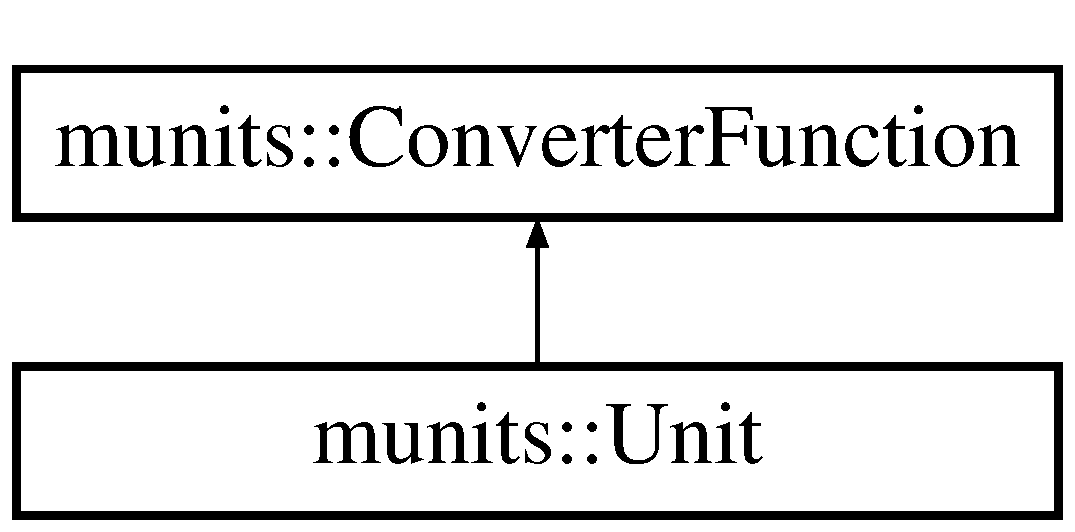
\includegraphics[height=2.000000cm]{classmunits_1_1_converter_function}
\end{center}
\end{figure}
\subsection*{Public Member Functions}
\begin{DoxyCompactItemize}
\item 
\hyperlink{classmunits_1_1_converter_function_ade93c9534fa3fdfea3e28012c4a35e71}{Converter\+Function} (double, double, const char $\ast$)
\item 
double \hyperlink{classmunits_1_1_converter_function_a4046b7450750f1becd45b63a811b14f0}{to\+\_\+base} (double, double) const
\item 
double \hyperlink{classmunits_1_1_converter_function_a06dfbd71248463c6d3d4b0cdda251612}{from\+\_\+base} (double, double) const
\item 
double \hyperlink{classmunits_1_1_converter_function_a1b3777fbb09c52bc9456fbae09295cfc}{get\+First\+Order\+Exponent} ()
\end{DoxyCompactItemize}


\subsection{Constructor \& Destructor Documentation}
\mbox{\Hypertarget{classmunits_1_1_converter_function_ade93c9534fa3fdfea3e28012c4a35e71}\label{classmunits_1_1_converter_function_ade93c9534fa3fdfea3e28012c4a35e71}} 
\index{munits\+::\+Converter\+Function@{munits\+::\+Converter\+Function}!Converter\+Function@{Converter\+Function}}
\index{Converter\+Function@{Converter\+Function}!munits\+::\+Converter\+Function@{munits\+::\+Converter\+Function}}
\subsubsection{\texorpdfstring{Converter\+Function()}{ConverterFunction()}}
{\footnotesize\ttfamily munits\+::\+Converter\+Function\+::\+Converter\+Function (\begin{DoxyParamCaption}\item[{double}]{a,  }\item[{double}]{b = {\ttfamily 0},  }\item[{const char $\ast$}]{s = {\ttfamily \char`\"{}Default\char`\"{}} }\end{DoxyParamCaption})\hspace{0.3cm}{\ttfamily [explicit]}}



\subsection{Member Function Documentation}
\mbox{\Hypertarget{classmunits_1_1_converter_function_a06dfbd71248463c6d3d4b0cdda251612}\label{classmunits_1_1_converter_function_a06dfbd71248463c6d3d4b0cdda251612}} 
\index{munits\+::\+Converter\+Function@{munits\+::\+Converter\+Function}!from\+\_\+base@{from\+\_\+base}}
\index{from\+\_\+base@{from\+\_\+base}!munits\+::\+Converter\+Function@{munits\+::\+Converter\+Function}}
\subsubsection{\texorpdfstring{from\+\_\+base()}{from\_base()}}
{\footnotesize\ttfamily double munits\+::\+Converter\+Function\+::from\+\_\+base (\begin{DoxyParamCaption}\item[{double}]{v,  }\item[{double}]{e = {\ttfamily 1} }\end{DoxyParamCaption}) const}

\mbox{\Hypertarget{classmunits_1_1_converter_function_a1b3777fbb09c52bc9456fbae09295cfc}\label{classmunits_1_1_converter_function_a1b3777fbb09c52bc9456fbae09295cfc}} 
\index{munits\+::\+Converter\+Function@{munits\+::\+Converter\+Function}!get\+First\+Order\+Exponent@{get\+First\+Order\+Exponent}}
\index{get\+First\+Order\+Exponent@{get\+First\+Order\+Exponent}!munits\+::\+Converter\+Function@{munits\+::\+Converter\+Function}}
\subsubsection{\texorpdfstring{get\+First\+Order\+Exponent()}{getFirstOrderExponent()}}
{\footnotesize\ttfamily double munits\+::\+Converter\+Function\+::get\+First\+Order\+Exponent (\begin{DoxyParamCaption}{ }\end{DoxyParamCaption})\hspace{0.3cm}{\ttfamily [inline]}}

\mbox{\Hypertarget{classmunits_1_1_converter_function_a4046b7450750f1becd45b63a811b14f0}\label{classmunits_1_1_converter_function_a4046b7450750f1becd45b63a811b14f0}} 
\index{munits\+::\+Converter\+Function@{munits\+::\+Converter\+Function}!to\+\_\+base@{to\+\_\+base}}
\index{to\+\_\+base@{to\+\_\+base}!munits\+::\+Converter\+Function@{munits\+::\+Converter\+Function}}
\subsubsection{\texorpdfstring{to\+\_\+base()}{to\_base()}}
{\footnotesize\ttfamily double munits\+::\+Converter\+Function\+::to\+\_\+base (\begin{DoxyParamCaption}\item[{double}]{v,  }\item[{double}]{e = {\ttfamily 1} }\end{DoxyParamCaption}) const}



The documentation for this class was generated from the following files\+:\begin{DoxyCompactItemize}
\item 
Z\+:/ocs\+\_\+1/measurmentunits/src/\hyperlink{converter__function_8hpp}{converter\+\_\+function.\+hpp}\item 
Z\+:/ocs\+\_\+1/measurmentunits/src/\hyperlink{converter__function_8cpp}{converter\+\_\+function.\+cpp}\end{DoxyCompactItemize}

\hypertarget{structmunits_1_1_metric}{}\section{munits\+:\+:Metric Struct Reference}
\label{structmunits_1_1_metric}\index{munits\+::\+Metric@{munits\+::\+Metric}}


{\ttfamily \#include $<$metric.\+hpp$>$}

\subsection*{Public Member Functions}
\begin{DoxyCompactItemize}
\item 
\hyperlink{structmunits_1_1_metric_a365db074d677d69008f3aa919faf2a09}{Metric} (std\+::vector$<$ int $>$, std\+::string=\char`\"{}\char`\"{}, std\+::set$<$ std\+::string $>$=std\+::set$<$ std\+::string $>$(), const std\+::map$<$ std\+::string, const std\+::shared\+\_\+ptr$<$ \hyperlink{classmunits_1_1_unit}{munits\+::\+Unit} $>$$>$=std\+::map$<$ std\+::string, const std\+::shared\+\_\+ptr$<$ \hyperlink{classmunits_1_1_unit}{munits\+::\+Unit} $>$$>$(), const std\+::map$<$ const std\+::string, const std\+::string $>$=std\+::map$<$ const std\+::string, const std\+::string $>$())
\end{DoxyCompactItemize}
\subsection*{Public Attributes}
\begin{DoxyCompactItemize}
\item 
const std\+::vector$<$ int $>$ \hyperlink{structmunits_1_1_metric_a4beffad44091db5d1173075b5130266d}{dim\+\_\+vector}
\item 
const std\+::shared\+\_\+ptr$<$ \hyperlink{classmunits_1_1_converter}{munits\+::\+Converter} $>$ \hyperlink{structmunits_1_1_metric_aa51faca2f90c8bc80a8c5144a1ce15a0}{converter}
\item 
const std\+::map$<$ const std\+::string, const std\+::string $>$ \hyperlink{structmunits_1_1_metric_aa44951fa72f8ba14225164eb518ea9ac}{unit\+\_\+resolve\+\_\+mapping}
\end{DoxyCompactItemize}


\subsection{Constructor \& Destructor Documentation}
\mbox{\Hypertarget{structmunits_1_1_metric_a365db074d677d69008f3aa919faf2a09}\label{structmunits_1_1_metric_a365db074d677d69008f3aa919faf2a09}} 
\index{munits\+::\+Metric@{munits\+::\+Metric}!Metric@{Metric}}
\index{Metric@{Metric}!munits\+::\+Metric@{munits\+::\+Metric}}
\subsubsection{\texorpdfstring{Metric()}{Metric()}}
{\footnotesize\ttfamily munits\+::\+Metric\+::\+Metric (\begin{DoxyParamCaption}\item[{std\+::vector$<$ int $>$}]{,  }\item[{std\+::string}]{ = {\ttfamily \char`\"{}\char`\"{}},  }\item[{std\+::set$<$ std\+::string $>$}]{ = {\ttfamily std\+:\+:set$<$std\+:\+:string$>$()},  }\item[{const std\+::map$<$ std\+::string, const std\+::shared\+\_\+ptr$<$ \hyperlink{classmunits_1_1_unit}{munits\+::\+Unit} $>$$>$}]{ = {\ttfamily std\+:\+:map$<$std\+:\+:string,~const~std\+:\+:shared\+\_\+ptr~$<$\hyperlink{classmunits_1_1_unit}{munits\+::\+Unit}$>$$>$()},  }\item[{const std\+::map$<$ const std\+::string, const std\+::string $>$}]{ = {\ttfamily std\+:\+:map$<$const~std\+:\+:string,~const~std\+:\+:string$>$()} }\end{DoxyParamCaption})}



\subsection{Member Data Documentation}
\mbox{\Hypertarget{structmunits_1_1_metric_aa51faca2f90c8bc80a8c5144a1ce15a0}\label{structmunits_1_1_metric_aa51faca2f90c8bc80a8c5144a1ce15a0}} 
\index{munits\+::\+Metric@{munits\+::\+Metric}!converter@{converter}}
\index{converter@{converter}!munits\+::\+Metric@{munits\+::\+Metric}}
\subsubsection{\texorpdfstring{converter}{converter}}
{\footnotesize\ttfamily const std\+::shared\+\_\+ptr$<$\hyperlink{classmunits_1_1_converter}{munits\+::\+Converter}$>$ munits\+::\+Metric\+::converter}

\mbox{\Hypertarget{structmunits_1_1_metric_a4beffad44091db5d1173075b5130266d}\label{structmunits_1_1_metric_a4beffad44091db5d1173075b5130266d}} 
\index{munits\+::\+Metric@{munits\+::\+Metric}!dim\+\_\+vector@{dim\+\_\+vector}}
\index{dim\+\_\+vector@{dim\+\_\+vector}!munits\+::\+Metric@{munits\+::\+Metric}}
\subsubsection{\texorpdfstring{dim\+\_\+vector}{dim\_vector}}
{\footnotesize\ttfamily const std\+::vector$<$int$>$ munits\+::\+Metric\+::dim\+\_\+vector}

\mbox{\Hypertarget{structmunits_1_1_metric_aa44951fa72f8ba14225164eb518ea9ac}\label{structmunits_1_1_metric_aa44951fa72f8ba14225164eb518ea9ac}} 
\index{munits\+::\+Metric@{munits\+::\+Metric}!unit\+\_\+resolve\+\_\+mapping@{unit\+\_\+resolve\+\_\+mapping}}
\index{unit\+\_\+resolve\+\_\+mapping@{unit\+\_\+resolve\+\_\+mapping}!munits\+::\+Metric@{munits\+::\+Metric}}
\subsubsection{\texorpdfstring{unit\+\_\+resolve\+\_\+mapping}{unit\_resolve\_mapping}}
{\footnotesize\ttfamily const std\+::map$<$const std\+::string, const std\+::string$>$ munits\+::\+Metric\+::unit\+\_\+resolve\+\_\+mapping}



The documentation for this struct was generated from the following files\+:\begin{DoxyCompactItemize}
\item 
Z\+:/ocs\+\_\+1/measurmentunits/src/\hyperlink{metric_8hpp}{metric.\+hpp}\item 
Z\+:/ocs\+\_\+1/measurmentunits/src/\hyperlink{metric_8cpp}{metric.\+cpp}\end{DoxyCompactItemize}

\hypertarget{classmunits_1_1_prefix}{}\section{munits\+:\+:Prefix Class Reference}
\label{classmunits_1_1_prefix}\index{munits\+::\+Prefix@{munits\+::\+Prefix}}


{\ttfamily \#include $<$prefix.\+hpp$>$}

\subsection*{Public Member Functions}
\begin{DoxyCompactItemize}
\item 
\hyperlink{classmunits_1_1_prefix_a4696b743ad2374b9833a0628c55733b8}{Prefix} (const std\+::string n, const \hyperlink{classmunits_1_1_converter_function}{munits\+::\+Converter\+Function} \&cf, int exp=1)
\item 
std\+::string \hyperlink{classmunits_1_1_prefix_a3cc3d1b3ed55c756b8baa98ea1369e65}{get\+Notation} ()
\end{DoxyCompactItemize}
\subsection*{Friends}
\begin{DoxyCompactItemize}
\item 
const friend std\+::ostream \& \hyperlink{classmunits_1_1_prefix_a6dfdc18ee1d503dce5f170b4b04afa36}{operator$<$$<$} (std\+::ostream \&str, const \hyperlink{classmunits_1_1_prefix}{Prefix} \&a)
\item 
\hyperlink{classmunits_1_1_unit_notation}{munits\+::\+Unit\+Notation} \hyperlink{classmunits_1_1_prefix_a69fa2333393cf327262c44ec78eef70b}{merge\+Prefix\+With\+Notation} (const \hyperlink{classmunits_1_1_prefix}{Prefix} \&prx, const \hyperlink{classmunits_1_1_unit_notation}{munits\+::\+Unit\+Notation} \&un, int \&overflow)
\end{DoxyCompactItemize}


\subsection{Constructor \& Destructor Documentation}
\mbox{\Hypertarget{classmunits_1_1_prefix_a4696b743ad2374b9833a0628c55733b8}\label{classmunits_1_1_prefix_a4696b743ad2374b9833a0628c55733b8}} 
\index{munits\+::\+Prefix@{munits\+::\+Prefix}!Prefix@{Prefix}}
\index{Prefix@{Prefix}!munits\+::\+Prefix@{munits\+::\+Prefix}}
\subsubsection{\texorpdfstring{Prefix()}{Prefix()}}
{\footnotesize\ttfamily munits\+::\+Prefix\+::\+Prefix (\begin{DoxyParamCaption}\item[{const std\+::string}]{n,  }\item[{const \hyperlink{classmunits_1_1_converter_function}{munits\+::\+Converter\+Function} \&}]{cf,  }\item[{int}]{exp = {\ttfamily 1} }\end{DoxyParamCaption})\hspace{0.3cm}{\ttfamily [inline]}}



\subsection{Member Function Documentation}
\mbox{\Hypertarget{classmunits_1_1_prefix_a3cc3d1b3ed55c756b8baa98ea1369e65}\label{classmunits_1_1_prefix_a3cc3d1b3ed55c756b8baa98ea1369e65}} 
\index{munits\+::\+Prefix@{munits\+::\+Prefix}!get\+Notation@{get\+Notation}}
\index{get\+Notation@{get\+Notation}!munits\+::\+Prefix@{munits\+::\+Prefix}}
\subsubsection{\texorpdfstring{get\+Notation()}{getNotation()}}
{\footnotesize\ttfamily std\+::string munits\+::\+Prefix\+::get\+Notation (\begin{DoxyParamCaption}{ }\end{DoxyParamCaption})\hspace{0.3cm}{\ttfamily [inline]}}



\subsection{Friends And Related Function Documentation}
\mbox{\Hypertarget{classmunits_1_1_prefix_a69fa2333393cf327262c44ec78eef70b}\label{classmunits_1_1_prefix_a69fa2333393cf327262c44ec78eef70b}} 
\index{munits\+::\+Prefix@{munits\+::\+Prefix}!merge\+Prefix\+With\+Notation@{merge\+Prefix\+With\+Notation}}
\index{merge\+Prefix\+With\+Notation@{merge\+Prefix\+With\+Notation}!munits\+::\+Prefix@{munits\+::\+Prefix}}
\subsubsection{\texorpdfstring{merge\+Prefix\+With\+Notation}{mergePrefixWithNotation}}
{\footnotesize\ttfamily \hyperlink{classmunits_1_1_unit_notation}{munits\+::\+Unit\+Notation} merge\+Prefix\+With\+Notation (\begin{DoxyParamCaption}\item[{const \hyperlink{classmunits_1_1_prefix}{Prefix} \&}]{prx,  }\item[{const \hyperlink{classmunits_1_1_unit_notation}{munits\+::\+Unit\+Notation} \&}]{un,  }\item[{int \&}]{overflow }\end{DoxyParamCaption})\hspace{0.3cm}{\ttfamily [friend]}}

\mbox{\Hypertarget{classmunits_1_1_prefix_a6dfdc18ee1d503dce5f170b4b04afa36}\label{classmunits_1_1_prefix_a6dfdc18ee1d503dce5f170b4b04afa36}} 
\index{munits\+::\+Prefix@{munits\+::\+Prefix}!operator$<$$<$@{operator$<$$<$}}
\index{operator$<$$<$@{operator$<$$<$}!munits\+::\+Prefix@{munits\+::\+Prefix}}
\subsubsection{\texorpdfstring{operator$<$$<$}{operator<<}}
{\footnotesize\ttfamily const friend std\+::ostream\& operator$<$$<$ (\begin{DoxyParamCaption}\item[{std\+::ostream \&}]{str,  }\item[{const \hyperlink{classmunits_1_1_prefix}{Prefix} \&}]{a }\end{DoxyParamCaption})\hspace{0.3cm}{\ttfamily [friend]}}



The documentation for this class was generated from the following file\+:\begin{DoxyCompactItemize}
\item 
Z\+:/ocs\+\_\+1/measurmentunits/src/\hyperlink{prefix_8hpp}{prefix.\+hpp}\end{DoxyCompactItemize}

\hypertarget{classmunits_1_1_quantity}{}\section{munits\+:\+:Quantity Class Reference}
\label{classmunits_1_1_quantity}\index{munits\+::\+Quantity@{munits\+::\+Quantity}}


{\ttfamily \#include $<$quantity.\+h$>$}

\subsection*{Public Member Functions}
\begin{DoxyCompactItemize}
\item 
const \hyperlink{classmunits_1_1_unit_notation_vector}{munits\+::\+Unit\+Notation\+Vector} \hyperlink{classmunits_1_1_quantity_ad9dadbbab677bf22170412595e65cc2f}{get\+Unit\+Vector} () const
\item 
\hyperlink{classmunits_1_1_quantity_a7b99d99300cfad3056e2b426644531eb}{Quantity} (\hyperlink{namespacemunits_a22c8effe19fdc3eb888884aa217f0c25}{metrics}, double, const std\+::string)
\item 
\hyperlink{classmunits_1_1_quantity_aeeb10868a2ec67f430442182b2690869}{Quantity} (const \hyperlink{classmunits_1_1_quantity}{Quantity} \&)=default
\item 
\hyperlink{classmunits_1_1_quantity}{Quantity} \& \hyperlink{classmunits_1_1_quantity_af77fd9cb9469a6b71c8a27004f5dabe4}{operator=} (const \hyperlink{classmunits_1_1_quantity}{Quantity} \&)=default
\item 
\hyperlink{classmunits_1_1_quantity_a01e795d566b95da5ecbe0f1aa99076d7}{$\sim$\+Quantity} ()
\item 
const std\+::vector$<$ int $>$ \hyperlink{classmunits_1_1_quantity_a3210eda57592da41b8894128bb0d6544}{Get\+Dim\+Vector} () const
\item 
const int \hyperlink{classmunits_1_1_quantity_a9167bbf331462dc79bfd62fec4a90f84}{get\+Matrix\+Index} () const
\item 
double \hyperlink{classmunits_1_1_quantity_ac9e9f65483a14ec729bb684d629091bc}{operator()} (const std\+::string) const
\item 
\hyperlink{classmunits_1_1_quantity_ad5d294ad29bf6faaf64ed1f9b92ba5e0}{operator std\+::string} () const
\item 
\hyperlink{classmunits_1_1_quantity_a57e30283ba53c0e942a1d01fe2061bd7}{operator double} () const
\item 
bool \hyperlink{classmunits_1_1_quantity_a09ed96601cab6f56278e3bf44dc82b70}{unquantified} () const
\item 
std\+::string \hyperlink{classmunits_1_1_quantity_a3f09b8e8dbd47f32a21f94591508c0fe}{to\+String} () const
\item 
double \hyperlink{classmunits_1_1_quantity_aadf35d14997bb3e58d8d2681f7c24ae3}{to\+Double} () const
\item 
double \hyperlink{classmunits_1_1_quantity_aae7dc378d4da3a9466edc958626f13d3}{get\+Value} () const
\item 
std\+::string \hyperlink{classmunits_1_1_quantity_a2de8a125226f981bf9a1d5a47b5957bb}{get\+Unit} () const
\item 
\hyperlink{classmunits_1_1_quantity_a0b43d7b58dbb07aca7382ef2630779d7}{Quantity} ()
\item 
\hyperlink{classmunits_1_1_quantity}{Quantity} \hyperlink{classmunits_1_1_quantity_aa46193a0c20d60713d279eb0b7a1da1f}{ntrt} (const int exponent) const
\end{DoxyCompactItemize}
\subsection*{Friends}
\begin{DoxyCompactItemize}
\item 
std\+::ostream \& \hyperlink{classmunits_1_1_quantity_a26328f678ccbddf64026c4f217938afb}{operator$<$$<$} (std\+::ostream \&str, const \hyperlink{classmunits_1_1_quantity}{Quantity} \&a)
\item 
\hyperlink{classmunits_1_1_quantity}{Quantity} \hyperlink{classmunits_1_1_quantity_a31795b0bdac61b168e21eb109d4f9909}{operator+} (const \hyperlink{classmunits_1_1_quantity}{Quantity} \&lfths, const \hyperlink{classmunits_1_1_quantity}{Quantity} \&rgths)
\item 
\hyperlink{classmunits_1_1_quantity}{Quantity} \hyperlink{classmunits_1_1_quantity_abcc9929246b92475a9008ed1a8b30160}{operator-\/} (const \hyperlink{classmunits_1_1_quantity}{Quantity} \&lfths, const \hyperlink{classmunits_1_1_quantity}{Quantity} \&rgths)
\item 
\hyperlink{classmunits_1_1_quantity}{Quantity} \hyperlink{classmunits_1_1_quantity_a590dff743167fea46e7b6e660fef0471}{operator$\ast$} (const \hyperlink{classmunits_1_1_quantity}{Quantity} \&lfths, const \hyperlink{classmunits_1_1_quantity}{Quantity} \&rgths)
\item 
\hyperlink{classmunits_1_1_quantity}{Quantity} \hyperlink{classmunits_1_1_quantity_a3b34f864a8d7dc26122650987a08db74}{operator$\ast$} (const \hyperlink{classmunits_1_1_quantity}{Quantity} \&lfths, const int rgths)
\item 
\hyperlink{classmunits_1_1_quantity}{Quantity} \hyperlink{classmunits_1_1_quantity_a537ae4feae57faf4d03626a02df64918}{operator$\ast$} (const int lfths, const \hyperlink{classmunits_1_1_quantity}{Quantity} \&rgths)
\item 
\hyperlink{classmunits_1_1_quantity}{Quantity} \hyperlink{classmunits_1_1_quantity_ab1bd381ef86466a48f2ed99d64a96141}{operator$\ast$} (const \hyperlink{classmunits_1_1_quantity}{Quantity} \&lfths, const double rgths)
\item 
\hyperlink{classmunits_1_1_quantity}{Quantity} \hyperlink{classmunits_1_1_quantity_a0f7ddd0457e20b83847135178d2d71f0}{operator$\ast$} (const double lfths, const \hyperlink{classmunits_1_1_quantity}{Quantity} \&rgths)
\item 
\hyperlink{classmunits_1_1_quantity}{Quantity} \hyperlink{classmunits_1_1_quantity_a7efa534b51546377b466e035f7ef1ea9}{operator/} (const \hyperlink{classmunits_1_1_quantity}{Quantity} \&lfths, const \hyperlink{classmunits_1_1_quantity}{Quantity} \&rgths)
\item 
\hyperlink{classmunits_1_1_quantity}{Quantity} \hyperlink{classmunits_1_1_quantity_a2854dec1ef94e67d8ff0e50900dceddc}{operator/} (const \hyperlink{classmunits_1_1_quantity}{Quantity} \&lfths, const int rgths)
\item 
\hyperlink{classmunits_1_1_quantity}{Quantity} \hyperlink{classmunits_1_1_quantity_a6a34ef12ca317a49f45c310ef232ee4e}{operator/} (const \hyperlink{classmunits_1_1_quantity}{Quantity} \&lfths, const double rgths)
\item 
bool \hyperlink{classmunits_1_1_quantity_a1b7db6ef3157f54dffd8431b73b059f9}{operator$<$} (const \hyperlink{classmunits_1_1_quantity}{Quantity} \&lfths, const \hyperlink{classmunits_1_1_quantity}{Quantity} \&rgths)
\item 
bool \hyperlink{classmunits_1_1_quantity_a6ddc2fc0e787211815087612a60c35d1}{operator$<$=} (const \hyperlink{classmunits_1_1_quantity}{Quantity} \&lfths, const \hyperlink{classmunits_1_1_quantity}{Quantity} \&rgths)
\item 
bool \hyperlink{classmunits_1_1_quantity_aa816c6e6e556d7f919273c67c287030b}{operator$>$} (const \hyperlink{classmunits_1_1_quantity}{Quantity} \&lfths, const \hyperlink{classmunits_1_1_quantity}{Quantity} \&rgths)
\item 
bool \hyperlink{classmunits_1_1_quantity_a700091f1868ef19f9bd02f289ac8a1ee}{operator$>$=} (const \hyperlink{classmunits_1_1_quantity}{Quantity} \&lfths, const \hyperlink{classmunits_1_1_quantity}{Quantity} \&rgths)
\item 
bool \hyperlink{classmunits_1_1_quantity_ab8fa0c93b87037ad0a27eec194454b60}{operator==} (const \hyperlink{classmunits_1_1_quantity}{Quantity} \&lfths, const \hyperlink{classmunits_1_1_quantity}{Quantity} \&rgths)
\item 
bool \hyperlink{classmunits_1_1_quantity_aa57bf85906856611bd00e12150faf573}{operator!=} (const \hyperlink{classmunits_1_1_quantity}{Quantity} \&lfths, const \hyperlink{classmunits_1_1_quantity}{Quantity} \&rgths)
\end{DoxyCompactItemize}


\subsection{Constructor \& Destructor Documentation}
\mbox{\Hypertarget{classmunits_1_1_quantity_a7b99d99300cfad3056e2b426644531eb}\label{classmunits_1_1_quantity_a7b99d99300cfad3056e2b426644531eb}} 
\index{munits\+::\+Quantity@{munits\+::\+Quantity}!Quantity@{Quantity}}
\index{Quantity@{Quantity}!munits\+::\+Quantity@{munits\+::\+Quantity}}
\subsubsection{\texorpdfstring{Quantity()}{Quantity()}\hspace{0.1cm}{\footnotesize\ttfamily [1/3]}}
{\footnotesize\ttfamily munits\+::\+Quantity\+::\+Quantity (\begin{DoxyParamCaption}\item[{\hyperlink{namespacemunits_a22c8effe19fdc3eb888884aa217f0c25}{metrics}}]{,  }\item[{double}]{,  }\item[{const std\+::string}]{ }\end{DoxyParamCaption})\hspace{0.3cm}{\ttfamily [explicit]}}

\mbox{\Hypertarget{classmunits_1_1_quantity_aeeb10868a2ec67f430442182b2690869}\label{classmunits_1_1_quantity_aeeb10868a2ec67f430442182b2690869}} 
\index{munits\+::\+Quantity@{munits\+::\+Quantity}!Quantity@{Quantity}}
\index{Quantity@{Quantity}!munits\+::\+Quantity@{munits\+::\+Quantity}}
\subsubsection{\texorpdfstring{Quantity()}{Quantity()}\hspace{0.1cm}{\footnotesize\ttfamily [2/3]}}
{\footnotesize\ttfamily munits\+::\+Quantity\+::\+Quantity (\begin{DoxyParamCaption}\item[{const \hyperlink{classmunits_1_1_quantity}{Quantity} \&}]{ }\end{DoxyParamCaption})\hspace{0.3cm}{\ttfamily [default]}}

\mbox{\Hypertarget{classmunits_1_1_quantity_a01e795d566b95da5ecbe0f1aa99076d7}\label{classmunits_1_1_quantity_a01e795d566b95da5ecbe0f1aa99076d7}} 
\index{munits\+::\+Quantity@{munits\+::\+Quantity}!````~Quantity@{$\sim$\+Quantity}}
\index{````~Quantity@{$\sim$\+Quantity}!munits\+::\+Quantity@{munits\+::\+Quantity}}
\subsubsection{\texorpdfstring{$\sim$\+Quantity()}{~Quantity()}}
{\footnotesize\ttfamily munits\+::\+Quantity\+::$\sim$\+Quantity (\begin{DoxyParamCaption}{ }\end{DoxyParamCaption})\hspace{0.3cm}{\ttfamily [inline]}}

\mbox{\Hypertarget{classmunits_1_1_quantity_a0b43d7b58dbb07aca7382ef2630779d7}\label{classmunits_1_1_quantity_a0b43d7b58dbb07aca7382ef2630779d7}} 
\index{munits\+::\+Quantity@{munits\+::\+Quantity}!Quantity@{Quantity}}
\index{Quantity@{Quantity}!munits\+::\+Quantity@{munits\+::\+Quantity}}
\subsubsection{\texorpdfstring{Quantity()}{Quantity()}\hspace{0.1cm}{\footnotesize\ttfamily [3/3]}}
{\footnotesize\ttfamily munits\+::\+Quantity\+::\+Quantity (\begin{DoxyParamCaption}{ }\end{DoxyParamCaption})\hspace{0.3cm}{\ttfamily [inline]}}



\subsection{Member Function Documentation}
\mbox{\Hypertarget{classmunits_1_1_quantity_a3210eda57592da41b8894128bb0d6544}\label{classmunits_1_1_quantity_a3210eda57592da41b8894128bb0d6544}} 
\index{munits\+::\+Quantity@{munits\+::\+Quantity}!Get\+Dim\+Vector@{Get\+Dim\+Vector}}
\index{Get\+Dim\+Vector@{Get\+Dim\+Vector}!munits\+::\+Quantity@{munits\+::\+Quantity}}
\subsubsection{\texorpdfstring{Get\+Dim\+Vector()}{GetDimVector()}}
{\footnotesize\ttfamily const std\+::vector$<$int$>$ munits\+::\+Quantity\+::\+Get\+Dim\+Vector (\begin{DoxyParamCaption}{ }\end{DoxyParamCaption}) const\hspace{0.3cm}{\ttfamily [inline]}}

\mbox{\Hypertarget{classmunits_1_1_quantity_a9167bbf331462dc79bfd62fec4a90f84}\label{classmunits_1_1_quantity_a9167bbf331462dc79bfd62fec4a90f84}} 
\index{munits\+::\+Quantity@{munits\+::\+Quantity}!get\+Matrix\+Index@{get\+Matrix\+Index}}
\index{get\+Matrix\+Index@{get\+Matrix\+Index}!munits\+::\+Quantity@{munits\+::\+Quantity}}
\subsubsection{\texorpdfstring{get\+Matrix\+Index()}{getMatrixIndex()}}
{\footnotesize\ttfamily const int munits\+::\+Quantity\+::get\+Matrix\+Index (\begin{DoxyParamCaption}{ }\end{DoxyParamCaption}) const\hspace{0.3cm}{\ttfamily [inline]}}

\mbox{\Hypertarget{classmunits_1_1_quantity_a2de8a125226f981bf9a1d5a47b5957bb}\label{classmunits_1_1_quantity_a2de8a125226f981bf9a1d5a47b5957bb}} 
\index{munits\+::\+Quantity@{munits\+::\+Quantity}!get\+Unit@{get\+Unit}}
\index{get\+Unit@{get\+Unit}!munits\+::\+Quantity@{munits\+::\+Quantity}}
\subsubsection{\texorpdfstring{get\+Unit()}{getUnit()}}
{\footnotesize\ttfamily std\+::string munits\+::\+Quantity\+::get\+Unit (\begin{DoxyParamCaption}{ }\end{DoxyParamCaption}) const\hspace{0.3cm}{\ttfamily [inline]}}

\mbox{\Hypertarget{classmunits_1_1_quantity_ad9dadbbab677bf22170412595e65cc2f}\label{classmunits_1_1_quantity_ad9dadbbab677bf22170412595e65cc2f}} 
\index{munits\+::\+Quantity@{munits\+::\+Quantity}!get\+Unit\+Vector@{get\+Unit\+Vector}}
\index{get\+Unit\+Vector@{get\+Unit\+Vector}!munits\+::\+Quantity@{munits\+::\+Quantity}}
\subsubsection{\texorpdfstring{get\+Unit\+Vector()}{getUnitVector()}}
{\footnotesize\ttfamily const \hyperlink{classmunits_1_1_unit_notation_vector}{munits\+::\+Unit\+Notation\+Vector} munits\+::\+Quantity\+::get\+Unit\+Vector (\begin{DoxyParamCaption}{ }\end{DoxyParamCaption}) const\hspace{0.3cm}{\ttfamily [inline]}}

\mbox{\Hypertarget{classmunits_1_1_quantity_aae7dc378d4da3a9466edc958626f13d3}\label{classmunits_1_1_quantity_aae7dc378d4da3a9466edc958626f13d3}} 
\index{munits\+::\+Quantity@{munits\+::\+Quantity}!get\+Value@{get\+Value}}
\index{get\+Value@{get\+Value}!munits\+::\+Quantity@{munits\+::\+Quantity}}
\subsubsection{\texorpdfstring{get\+Value()}{getValue()}}
{\footnotesize\ttfamily double munits\+::\+Quantity\+::get\+Value (\begin{DoxyParamCaption}{ }\end{DoxyParamCaption}) const\hspace{0.3cm}{\ttfamily [inline]}}

\mbox{\Hypertarget{classmunits_1_1_quantity_aa46193a0c20d60713d279eb0b7a1da1f}\label{classmunits_1_1_quantity_aa46193a0c20d60713d279eb0b7a1da1f}} 
\index{munits\+::\+Quantity@{munits\+::\+Quantity}!ntrt@{ntrt}}
\index{ntrt@{ntrt}!munits\+::\+Quantity@{munits\+::\+Quantity}}
\subsubsection{\texorpdfstring{ntrt()}{ntrt()}}
{\footnotesize\ttfamily \hyperlink{classmunits_1_1_quantity}{munits\+::\+Quantity} munits\+::\+Quantity\+::ntrt (\begin{DoxyParamCaption}\item[{const int}]{exponent }\end{DoxyParamCaption}) const}

\mbox{\Hypertarget{classmunits_1_1_quantity_a57e30283ba53c0e942a1d01fe2061bd7}\label{classmunits_1_1_quantity_a57e30283ba53c0e942a1d01fe2061bd7}} 
\index{munits\+::\+Quantity@{munits\+::\+Quantity}!operator double@{operator double}}
\index{operator double@{operator double}!munits\+::\+Quantity@{munits\+::\+Quantity}}
\subsubsection{\texorpdfstring{operator double()}{operator double()}}
{\footnotesize\ttfamily munits\+::\+Quantity\+::operator double (\begin{DoxyParamCaption}{ }\end{DoxyParamCaption}) const\hspace{0.3cm}{\ttfamily [explicit]}}

\mbox{\Hypertarget{classmunits_1_1_quantity_ad5d294ad29bf6faaf64ed1f9b92ba5e0}\label{classmunits_1_1_quantity_ad5d294ad29bf6faaf64ed1f9b92ba5e0}} 
\index{munits\+::\+Quantity@{munits\+::\+Quantity}!operator std\+::string@{operator std\+::string}}
\index{operator std\+::string@{operator std\+::string}!munits\+::\+Quantity@{munits\+::\+Quantity}}
\subsubsection{\texorpdfstring{operator std\+::string()}{operator std::string()}}
{\footnotesize\ttfamily munits\+::\+Quantity\+::operator std\+::string (\begin{DoxyParamCaption}{ }\end{DoxyParamCaption}) const\hspace{0.3cm}{\ttfamily [inline]}}

\mbox{\Hypertarget{classmunits_1_1_quantity_ac9e9f65483a14ec729bb684d629091bc}\label{classmunits_1_1_quantity_ac9e9f65483a14ec729bb684d629091bc}} 
\index{munits\+::\+Quantity@{munits\+::\+Quantity}!operator()@{operator()}}
\index{operator()@{operator()}!munits\+::\+Quantity@{munits\+::\+Quantity}}
\subsubsection{\texorpdfstring{operator()()}{operator()()}}
{\footnotesize\ttfamily double munits\+::\+Quantity\+::operator() (\begin{DoxyParamCaption}\item[{const std\+::string}]{ }\end{DoxyParamCaption}) const}

\mbox{\Hypertarget{classmunits_1_1_quantity_af77fd9cb9469a6b71c8a27004f5dabe4}\label{classmunits_1_1_quantity_af77fd9cb9469a6b71c8a27004f5dabe4}} 
\index{munits\+::\+Quantity@{munits\+::\+Quantity}!operator=@{operator=}}
\index{operator=@{operator=}!munits\+::\+Quantity@{munits\+::\+Quantity}}
\subsubsection{\texorpdfstring{operator=()}{operator=()}}
{\footnotesize\ttfamily \hyperlink{classmunits_1_1_quantity}{Quantity}\& munits\+::\+Quantity\+::operator= (\begin{DoxyParamCaption}\item[{const \hyperlink{classmunits_1_1_quantity}{Quantity} \&}]{ }\end{DoxyParamCaption})\hspace{0.3cm}{\ttfamily [default]}}

\mbox{\Hypertarget{classmunits_1_1_quantity_aadf35d14997bb3e58d8d2681f7c24ae3}\label{classmunits_1_1_quantity_aadf35d14997bb3e58d8d2681f7c24ae3}} 
\index{munits\+::\+Quantity@{munits\+::\+Quantity}!to\+Double@{to\+Double}}
\index{to\+Double@{to\+Double}!munits\+::\+Quantity@{munits\+::\+Quantity}}
\subsubsection{\texorpdfstring{to\+Double()}{toDouble()}}
{\footnotesize\ttfamily double munits\+::\+Quantity\+::to\+Double (\begin{DoxyParamCaption}{ }\end{DoxyParamCaption}) const\hspace{0.3cm}{\ttfamily [inline]}}

\mbox{\Hypertarget{classmunits_1_1_quantity_a3f09b8e8dbd47f32a21f94591508c0fe}\label{classmunits_1_1_quantity_a3f09b8e8dbd47f32a21f94591508c0fe}} 
\index{munits\+::\+Quantity@{munits\+::\+Quantity}!to\+String@{to\+String}}
\index{to\+String@{to\+String}!munits\+::\+Quantity@{munits\+::\+Quantity}}
\subsubsection{\texorpdfstring{to\+String()}{toString()}}
{\footnotesize\ttfamily std\+::string munits\+::\+Quantity\+::to\+String (\begin{DoxyParamCaption}{ }\end{DoxyParamCaption}) const\hspace{0.3cm}{\ttfamily [inline]}}

\mbox{\Hypertarget{classmunits_1_1_quantity_a09ed96601cab6f56278e3bf44dc82b70}\label{classmunits_1_1_quantity_a09ed96601cab6f56278e3bf44dc82b70}} 
\index{munits\+::\+Quantity@{munits\+::\+Quantity}!unquantified@{unquantified}}
\index{unquantified@{unquantified}!munits\+::\+Quantity@{munits\+::\+Quantity}}
\subsubsection{\texorpdfstring{unquantified()}{unquantified()}}
{\footnotesize\ttfamily bool munits\+::\+Quantity\+::unquantified (\begin{DoxyParamCaption}{ }\end{DoxyParamCaption}) const}



\subsection{Friends And Related Function Documentation}
\mbox{\Hypertarget{classmunits_1_1_quantity_aa57bf85906856611bd00e12150faf573}\label{classmunits_1_1_quantity_aa57bf85906856611bd00e12150faf573}} 
\index{munits\+::\+Quantity@{munits\+::\+Quantity}!operator"!=@{operator"!=}}
\index{operator"!=@{operator"!=}!munits\+::\+Quantity@{munits\+::\+Quantity}}
\subsubsection{\texorpdfstring{operator"!=}{operator!=}}
{\footnotesize\ttfamily bool operator!= (\begin{DoxyParamCaption}\item[{const \hyperlink{classmunits_1_1_quantity}{Quantity} \&}]{lfths,  }\item[{const \hyperlink{classmunits_1_1_quantity}{Quantity} \&}]{rgths }\end{DoxyParamCaption})\hspace{0.3cm}{\ttfamily [friend]}}

\mbox{\Hypertarget{classmunits_1_1_quantity_a590dff743167fea46e7b6e660fef0471}\label{classmunits_1_1_quantity_a590dff743167fea46e7b6e660fef0471}} 
\index{munits\+::\+Quantity@{munits\+::\+Quantity}!operator$\ast$@{operator$\ast$}}
\index{operator$\ast$@{operator$\ast$}!munits\+::\+Quantity@{munits\+::\+Quantity}}
\subsubsection{\texorpdfstring{operator$\ast$}{operator*}\hspace{0.1cm}{\footnotesize\ttfamily [1/5]}}
{\footnotesize\ttfamily \hyperlink{classmunits_1_1_quantity}{Quantity} operator$\ast$ (\begin{DoxyParamCaption}\item[{const \hyperlink{classmunits_1_1_quantity}{Quantity} \&}]{lfths,  }\item[{const \hyperlink{classmunits_1_1_quantity}{Quantity} \&}]{rgths }\end{DoxyParamCaption})\hspace{0.3cm}{\ttfamily [friend]}}

\mbox{\Hypertarget{classmunits_1_1_quantity_a3b34f864a8d7dc26122650987a08db74}\label{classmunits_1_1_quantity_a3b34f864a8d7dc26122650987a08db74}} 
\index{munits\+::\+Quantity@{munits\+::\+Quantity}!operator$\ast$@{operator$\ast$}}
\index{operator$\ast$@{operator$\ast$}!munits\+::\+Quantity@{munits\+::\+Quantity}}
\subsubsection{\texorpdfstring{operator$\ast$}{operator*}\hspace{0.1cm}{\footnotesize\ttfamily [2/5]}}
{\footnotesize\ttfamily \hyperlink{classmunits_1_1_quantity}{Quantity} operator$\ast$ (\begin{DoxyParamCaption}\item[{const \hyperlink{classmunits_1_1_quantity}{Quantity} \&}]{lfths,  }\item[{const int}]{rgths }\end{DoxyParamCaption})\hspace{0.3cm}{\ttfamily [friend]}}

\mbox{\Hypertarget{classmunits_1_1_quantity_a537ae4feae57faf4d03626a02df64918}\label{classmunits_1_1_quantity_a537ae4feae57faf4d03626a02df64918}} 
\index{munits\+::\+Quantity@{munits\+::\+Quantity}!operator$\ast$@{operator$\ast$}}
\index{operator$\ast$@{operator$\ast$}!munits\+::\+Quantity@{munits\+::\+Quantity}}
\subsubsection{\texorpdfstring{operator$\ast$}{operator*}\hspace{0.1cm}{\footnotesize\ttfamily [3/5]}}
{\footnotesize\ttfamily \hyperlink{classmunits_1_1_quantity}{Quantity} operator$\ast$ (\begin{DoxyParamCaption}\item[{const int}]{lfths,  }\item[{const \hyperlink{classmunits_1_1_quantity}{Quantity} \&}]{rgths }\end{DoxyParamCaption})\hspace{0.3cm}{\ttfamily [friend]}}

\mbox{\Hypertarget{classmunits_1_1_quantity_ab1bd381ef86466a48f2ed99d64a96141}\label{classmunits_1_1_quantity_ab1bd381ef86466a48f2ed99d64a96141}} 
\index{munits\+::\+Quantity@{munits\+::\+Quantity}!operator$\ast$@{operator$\ast$}}
\index{operator$\ast$@{operator$\ast$}!munits\+::\+Quantity@{munits\+::\+Quantity}}
\subsubsection{\texorpdfstring{operator$\ast$}{operator*}\hspace{0.1cm}{\footnotesize\ttfamily [4/5]}}
{\footnotesize\ttfamily \hyperlink{classmunits_1_1_quantity}{Quantity} operator$\ast$ (\begin{DoxyParamCaption}\item[{const \hyperlink{classmunits_1_1_quantity}{Quantity} \&}]{lfths,  }\item[{const double}]{rgths }\end{DoxyParamCaption})\hspace{0.3cm}{\ttfamily [friend]}}

\mbox{\Hypertarget{classmunits_1_1_quantity_a0f7ddd0457e20b83847135178d2d71f0}\label{classmunits_1_1_quantity_a0f7ddd0457e20b83847135178d2d71f0}} 
\index{munits\+::\+Quantity@{munits\+::\+Quantity}!operator$\ast$@{operator$\ast$}}
\index{operator$\ast$@{operator$\ast$}!munits\+::\+Quantity@{munits\+::\+Quantity}}
\subsubsection{\texorpdfstring{operator$\ast$}{operator*}\hspace{0.1cm}{\footnotesize\ttfamily [5/5]}}
{\footnotesize\ttfamily \hyperlink{classmunits_1_1_quantity}{Quantity} operator$\ast$ (\begin{DoxyParamCaption}\item[{const double}]{lfths,  }\item[{const \hyperlink{classmunits_1_1_quantity}{Quantity} \&}]{rgths }\end{DoxyParamCaption})\hspace{0.3cm}{\ttfamily [friend]}}

\mbox{\Hypertarget{classmunits_1_1_quantity_a31795b0bdac61b168e21eb109d4f9909}\label{classmunits_1_1_quantity_a31795b0bdac61b168e21eb109d4f9909}} 
\index{munits\+::\+Quantity@{munits\+::\+Quantity}!operator+@{operator+}}
\index{operator+@{operator+}!munits\+::\+Quantity@{munits\+::\+Quantity}}
\subsubsection{\texorpdfstring{operator+}{operator+}}
{\footnotesize\ttfamily \hyperlink{classmunits_1_1_quantity}{Quantity} operator+ (\begin{DoxyParamCaption}\item[{const \hyperlink{classmunits_1_1_quantity}{Quantity} \&}]{lfths,  }\item[{const \hyperlink{classmunits_1_1_quantity}{Quantity} \&}]{rgths }\end{DoxyParamCaption})\hspace{0.3cm}{\ttfamily [friend]}}

\mbox{\Hypertarget{classmunits_1_1_quantity_abcc9929246b92475a9008ed1a8b30160}\label{classmunits_1_1_quantity_abcc9929246b92475a9008ed1a8b30160}} 
\index{munits\+::\+Quantity@{munits\+::\+Quantity}!operator-\/@{operator-\/}}
\index{operator-\/@{operator-\/}!munits\+::\+Quantity@{munits\+::\+Quantity}}
\subsubsection{\texorpdfstring{operator-\/}{operator-}}
{\footnotesize\ttfamily \hyperlink{classmunits_1_1_quantity}{Quantity} operator-\/ (\begin{DoxyParamCaption}\item[{const \hyperlink{classmunits_1_1_quantity}{Quantity} \&}]{lfths,  }\item[{const \hyperlink{classmunits_1_1_quantity}{Quantity} \&}]{rgths }\end{DoxyParamCaption})\hspace{0.3cm}{\ttfamily [friend]}}

\mbox{\Hypertarget{classmunits_1_1_quantity_a7efa534b51546377b466e035f7ef1ea9}\label{classmunits_1_1_quantity_a7efa534b51546377b466e035f7ef1ea9}} 
\index{munits\+::\+Quantity@{munits\+::\+Quantity}!operator/@{operator/}}
\index{operator/@{operator/}!munits\+::\+Quantity@{munits\+::\+Quantity}}
\subsubsection{\texorpdfstring{operator/}{operator/}\hspace{0.1cm}{\footnotesize\ttfamily [1/3]}}
{\footnotesize\ttfamily \hyperlink{classmunits_1_1_quantity}{Quantity} operator/ (\begin{DoxyParamCaption}\item[{const \hyperlink{classmunits_1_1_quantity}{Quantity} \&}]{lfths,  }\item[{const \hyperlink{classmunits_1_1_quantity}{Quantity} \&}]{rgths }\end{DoxyParamCaption})\hspace{0.3cm}{\ttfamily [friend]}}

\mbox{\Hypertarget{classmunits_1_1_quantity_a2854dec1ef94e67d8ff0e50900dceddc}\label{classmunits_1_1_quantity_a2854dec1ef94e67d8ff0e50900dceddc}} 
\index{munits\+::\+Quantity@{munits\+::\+Quantity}!operator/@{operator/}}
\index{operator/@{operator/}!munits\+::\+Quantity@{munits\+::\+Quantity}}
\subsubsection{\texorpdfstring{operator/}{operator/}\hspace{0.1cm}{\footnotesize\ttfamily [2/3]}}
{\footnotesize\ttfamily \hyperlink{classmunits_1_1_quantity}{Quantity} operator/ (\begin{DoxyParamCaption}\item[{const \hyperlink{classmunits_1_1_quantity}{Quantity} \&}]{lfths,  }\item[{const int}]{rgths }\end{DoxyParamCaption})\hspace{0.3cm}{\ttfamily [friend]}}

\mbox{\Hypertarget{classmunits_1_1_quantity_a6a34ef12ca317a49f45c310ef232ee4e}\label{classmunits_1_1_quantity_a6a34ef12ca317a49f45c310ef232ee4e}} 
\index{munits\+::\+Quantity@{munits\+::\+Quantity}!operator/@{operator/}}
\index{operator/@{operator/}!munits\+::\+Quantity@{munits\+::\+Quantity}}
\subsubsection{\texorpdfstring{operator/}{operator/}\hspace{0.1cm}{\footnotesize\ttfamily [3/3]}}
{\footnotesize\ttfamily \hyperlink{classmunits_1_1_quantity}{Quantity} operator/ (\begin{DoxyParamCaption}\item[{const \hyperlink{classmunits_1_1_quantity}{Quantity} \&}]{lfths,  }\item[{const double}]{rgths }\end{DoxyParamCaption})\hspace{0.3cm}{\ttfamily [friend]}}

\mbox{\Hypertarget{classmunits_1_1_quantity_a1b7db6ef3157f54dffd8431b73b059f9}\label{classmunits_1_1_quantity_a1b7db6ef3157f54dffd8431b73b059f9}} 
\index{munits\+::\+Quantity@{munits\+::\+Quantity}!operator$<$@{operator$<$}}
\index{operator$<$@{operator$<$}!munits\+::\+Quantity@{munits\+::\+Quantity}}
\subsubsection{\texorpdfstring{operator$<$}{operator<}}
{\footnotesize\ttfamily bool operator$<$ (\begin{DoxyParamCaption}\item[{const \hyperlink{classmunits_1_1_quantity}{Quantity} \&}]{lfths,  }\item[{const \hyperlink{classmunits_1_1_quantity}{Quantity} \&}]{rgths }\end{DoxyParamCaption})\hspace{0.3cm}{\ttfamily [friend]}}

\mbox{\Hypertarget{classmunits_1_1_quantity_a26328f678ccbddf64026c4f217938afb}\label{classmunits_1_1_quantity_a26328f678ccbddf64026c4f217938afb}} 
\index{munits\+::\+Quantity@{munits\+::\+Quantity}!operator$<$$<$@{operator$<$$<$}}
\index{operator$<$$<$@{operator$<$$<$}!munits\+::\+Quantity@{munits\+::\+Quantity}}
\subsubsection{\texorpdfstring{operator$<$$<$}{operator<<}}
{\footnotesize\ttfamily std\+::ostream\& operator$<$$<$ (\begin{DoxyParamCaption}\item[{std\+::ostream \&}]{str,  }\item[{const \hyperlink{classmunits_1_1_quantity}{Quantity} \&}]{a }\end{DoxyParamCaption})\hspace{0.3cm}{\ttfamily [friend]}}

\mbox{\Hypertarget{classmunits_1_1_quantity_a6ddc2fc0e787211815087612a60c35d1}\label{classmunits_1_1_quantity_a6ddc2fc0e787211815087612a60c35d1}} 
\index{munits\+::\+Quantity@{munits\+::\+Quantity}!operator$<$=@{operator$<$=}}
\index{operator$<$=@{operator$<$=}!munits\+::\+Quantity@{munits\+::\+Quantity}}
\subsubsection{\texorpdfstring{operator$<$=}{operator<=}}
{\footnotesize\ttfamily bool operator$<$= (\begin{DoxyParamCaption}\item[{const \hyperlink{classmunits_1_1_quantity}{Quantity} \&}]{lfths,  }\item[{const \hyperlink{classmunits_1_1_quantity}{Quantity} \&}]{rgths }\end{DoxyParamCaption})\hspace{0.3cm}{\ttfamily [friend]}}

\mbox{\Hypertarget{classmunits_1_1_quantity_ab8fa0c93b87037ad0a27eec194454b60}\label{classmunits_1_1_quantity_ab8fa0c93b87037ad0a27eec194454b60}} 
\index{munits\+::\+Quantity@{munits\+::\+Quantity}!operator==@{operator==}}
\index{operator==@{operator==}!munits\+::\+Quantity@{munits\+::\+Quantity}}
\subsubsection{\texorpdfstring{operator==}{operator==}}
{\footnotesize\ttfamily bool operator== (\begin{DoxyParamCaption}\item[{const \hyperlink{classmunits_1_1_quantity}{Quantity} \&}]{lfths,  }\item[{const \hyperlink{classmunits_1_1_quantity}{Quantity} \&}]{rgths }\end{DoxyParamCaption})\hspace{0.3cm}{\ttfamily [friend]}}

\mbox{\Hypertarget{classmunits_1_1_quantity_aa816c6e6e556d7f919273c67c287030b}\label{classmunits_1_1_quantity_aa816c6e6e556d7f919273c67c287030b}} 
\index{munits\+::\+Quantity@{munits\+::\+Quantity}!operator$>$@{operator$>$}}
\index{operator$>$@{operator$>$}!munits\+::\+Quantity@{munits\+::\+Quantity}}
\subsubsection{\texorpdfstring{operator$>$}{operator>}}
{\footnotesize\ttfamily bool operator$>$ (\begin{DoxyParamCaption}\item[{const \hyperlink{classmunits_1_1_quantity}{Quantity} \&}]{lfths,  }\item[{const \hyperlink{classmunits_1_1_quantity}{Quantity} \&}]{rgths }\end{DoxyParamCaption})\hspace{0.3cm}{\ttfamily [friend]}}

\mbox{\Hypertarget{classmunits_1_1_quantity_a700091f1868ef19f9bd02f289ac8a1ee}\label{classmunits_1_1_quantity_a700091f1868ef19f9bd02f289ac8a1ee}} 
\index{munits\+::\+Quantity@{munits\+::\+Quantity}!operator$>$=@{operator$>$=}}
\index{operator$>$=@{operator$>$=}!munits\+::\+Quantity@{munits\+::\+Quantity}}
\subsubsection{\texorpdfstring{operator$>$=}{operator>=}}
{\footnotesize\ttfamily bool operator$>$= (\begin{DoxyParamCaption}\item[{const \hyperlink{classmunits_1_1_quantity}{Quantity} \&}]{lfths,  }\item[{const \hyperlink{classmunits_1_1_quantity}{Quantity} \&}]{rgths }\end{DoxyParamCaption})\hspace{0.3cm}{\ttfamily [friend]}}



The documentation for this class was generated from the following files\+:\begin{DoxyCompactItemize}
\item 
Z\+:/ocs\+\_\+1/measurmentunits/src/\hyperlink{quantity_8h}{quantity.\+h}\item 
Z\+:/ocs\+\_\+1/measurmentunits/src/\hyperlink{quantity_8cpp}{quantity.\+cpp}\end{DoxyCompactItemize}

\hypertarget{classmunits_1_1_resolver}{}\section{munits\+:\+:Resolver Class Reference}
\label{classmunits_1_1_resolver}\index{munits\+::\+Resolver@{munits\+::\+Resolver}}


{\ttfamily \#include $<$uresolver.\+hpp$>$}

\subsection*{Public Member Functions}
\begin{DoxyCompactItemize}
\item 
\hyperlink{classmunits_1_1_resolver_a7c5d7929af94f1edb1041efc70298ab2}{Resolver} (const std\+::vector$<$ \hyperlink{structmunits_1_1_metric}{munits\+::\+Metric} $>$ \&matrix=\hyperlink{namespacemunits_a8bf80780c6ef4ce5b588d266a2de306e}{munits\+::\+Get\+Matrix}(), const std\+::map$<$ std\+::string, const std\+::shared\+\_\+ptr$<$ \hyperlink{classmunits_1_1_converter_function}{munits\+::\+Converter\+Function} $>$$>$ \&prefixes=\hyperlink{namespacemunits_a43150beff0a68af86df9d5a02e69b334}{munits\+::\+Get\+Prefixes}())
\item 
bool \hyperlink{classmunits_1_1_resolver_a07c4a19ce9774fe126907482e108e811}{resolve} (std\+::list$<$ std\+::string $>$ \&l)
\end{DoxyCompactItemize}
\subsection*{Protected Attributes}
\begin{DoxyCompactItemize}
\item 
const std\+::vector$<$ \hyperlink{structmunits_1_1_metric}{munits\+::\+Metric} $>$ \& \hyperlink{classmunits_1_1_resolver_a08d9cca2538741f5931b108072c60888}{rmatrix}
\item 
const std\+::map$<$ std\+::string, const std\+::shared\+\_\+ptr$<$ \hyperlink{classmunits_1_1_converter_function}{munits\+::\+Converter\+Function} $>$ $>$ \& \hyperlink{classmunits_1_1_resolver_ad7d28db5df350e57ecda95aaae2a2e35}{rprefixes}
\end{DoxyCompactItemize}


\subsection{Constructor \& Destructor Documentation}
\mbox{\Hypertarget{classmunits_1_1_resolver_a7c5d7929af94f1edb1041efc70298ab2}\label{classmunits_1_1_resolver_a7c5d7929af94f1edb1041efc70298ab2}} 
\index{munits\+::\+Resolver@{munits\+::\+Resolver}!Resolver@{Resolver}}
\index{Resolver@{Resolver}!munits\+::\+Resolver@{munits\+::\+Resolver}}
\subsubsection{\texorpdfstring{Resolver()}{Resolver()}}
{\footnotesize\ttfamily munits\+::\+Resolver\+::\+Resolver (\begin{DoxyParamCaption}\item[{const std\+::vector$<$ \hyperlink{structmunits_1_1_metric}{munits\+::\+Metric} $>$ \&}]{matrix = {\ttfamily \hyperlink{namespacemunits_a8bf80780c6ef4ce5b588d266a2de306e}{munits\+::\+Get\+Matrix}()},  }\item[{const std\+::map$<$ std\+::string, const std\+::shared\+\_\+ptr$<$ \hyperlink{classmunits_1_1_converter_function}{munits\+::\+Converter\+Function} $>$$>$ \&}]{prefixes = {\ttfamily \hyperlink{namespacemunits_a43150beff0a68af86df9d5a02e69b334}{munits\+::\+Get\+Prefixes}()} }\end{DoxyParamCaption})\hspace{0.3cm}{\ttfamily [inline]}}



\subsection{Member Function Documentation}
\mbox{\Hypertarget{classmunits_1_1_resolver_a07c4a19ce9774fe126907482e108e811}\label{classmunits_1_1_resolver_a07c4a19ce9774fe126907482e108e811}} 
\index{munits\+::\+Resolver@{munits\+::\+Resolver}!resolve@{resolve}}
\index{resolve@{resolve}!munits\+::\+Resolver@{munits\+::\+Resolver}}
\subsubsection{\texorpdfstring{resolve()}{resolve()}}
{\footnotesize\ttfamily bool munits\+::\+Resolver\+::resolve (\begin{DoxyParamCaption}\item[{std\+::list$<$ std\+::string $>$ \&}]{l }\end{DoxyParamCaption})}



\subsection{Member Data Documentation}
\mbox{\Hypertarget{classmunits_1_1_resolver_a08d9cca2538741f5931b108072c60888}\label{classmunits_1_1_resolver_a08d9cca2538741f5931b108072c60888}} 
\index{munits\+::\+Resolver@{munits\+::\+Resolver}!rmatrix@{rmatrix}}
\index{rmatrix@{rmatrix}!munits\+::\+Resolver@{munits\+::\+Resolver}}
\subsubsection{\texorpdfstring{rmatrix}{rmatrix}}
{\footnotesize\ttfamily const std\+::vector$<$\hyperlink{structmunits_1_1_metric}{munits\+::\+Metric}$>$\& munits\+::\+Resolver\+::rmatrix\hspace{0.3cm}{\ttfamily [protected]}}

\mbox{\Hypertarget{classmunits_1_1_resolver_ad7d28db5df350e57ecda95aaae2a2e35}\label{classmunits_1_1_resolver_ad7d28db5df350e57ecda95aaae2a2e35}} 
\index{munits\+::\+Resolver@{munits\+::\+Resolver}!rprefixes@{rprefixes}}
\index{rprefixes@{rprefixes}!munits\+::\+Resolver@{munits\+::\+Resolver}}
\subsubsection{\texorpdfstring{rprefixes}{rprefixes}}
{\footnotesize\ttfamily const std\+::map$<$std\+::string, const std\+::shared\+\_\+ptr$<$\hyperlink{classmunits_1_1_converter_function}{munits\+::\+Converter\+Function}$>$ $>$\& munits\+::\+Resolver\+::rprefixes\hspace{0.3cm}{\ttfamily [protected]}}



The documentation for this class was generated from the following files\+:\begin{DoxyCompactItemize}
\item 
Z\+:/ocs\+\_\+1/measurmentunits/src/\hyperlink{uresolver_8hpp}{uresolver.\+hpp}\item 
Z\+:/ocs\+\_\+1/measurmentunits/src/\hyperlink{uresolver_8cpp}{uresolver.\+cpp}\end{DoxyCompactItemize}

\hypertarget{classmunits_1_1_unit}{}\section{munits\+:\+:Unit Class Reference}
\label{classmunits_1_1_unit}\index{munits\+::\+Unit@{munits\+::\+Unit}}


{\ttfamily \#include $<$unit.\+hpp$>$}

Inheritance diagram for munits\+:\+:Unit\+:\begin{figure}[H]
\begin{center}
\leavevmode
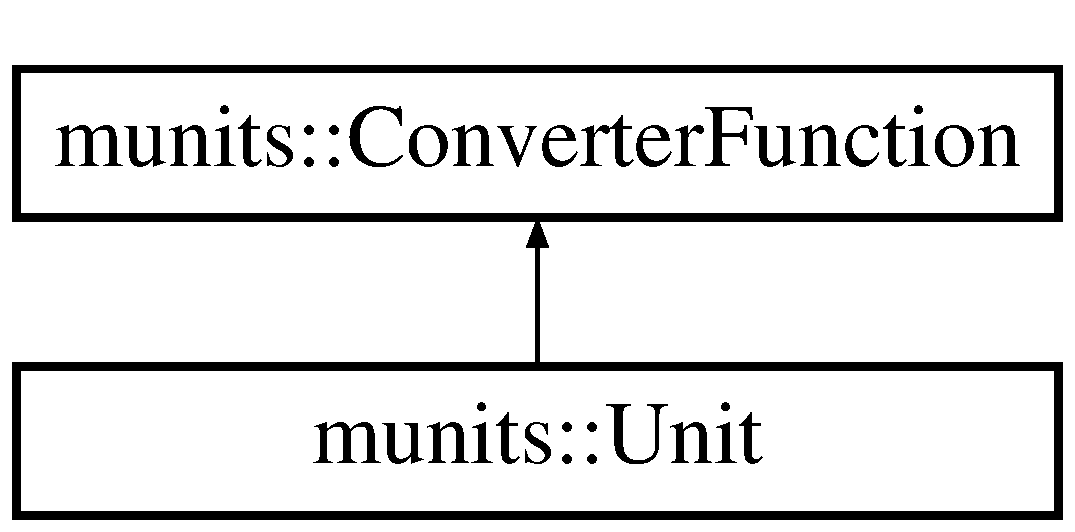
\includegraphics[height=2.000000cm]{classmunits_1_1_unit}
\end{center}
\end{figure}
\subsection*{Public Member Functions}
\begin{DoxyCompactItemize}
\item 
\hyperlink{classmunits_1_1_unit_a5e21dcab6e2e796ef1685c2c7ec70222}{Unit} (double a=1, double b=0, const char $\ast$s=\char`\"{}Default\char`\"{}, bool \hyperlink{classmunits_1_1_unit_a83a409eaa2d8bcb5940d90488f41bfbf}{applay\+\_\+prefix}=true, bool \hyperlink{classmunits_1_1_unit_a52145682ed514d15c6a79e0f6d9c2c90}{ignor\+\_\+exponent}=false)
\end{DoxyCompactItemize}
\subsection*{Public Attributes}
\begin{DoxyCompactItemize}
\item 
const bool \hyperlink{classmunits_1_1_unit_a83a409eaa2d8bcb5940d90488f41bfbf}{applay\+\_\+prefix}
\item 
const bool \hyperlink{classmunits_1_1_unit_a52145682ed514d15c6a79e0f6d9c2c90}{ignor\+\_\+exponent}
\end{DoxyCompactItemize}


\subsection{Constructor \& Destructor Documentation}
\mbox{\Hypertarget{classmunits_1_1_unit_a5e21dcab6e2e796ef1685c2c7ec70222}\label{classmunits_1_1_unit_a5e21dcab6e2e796ef1685c2c7ec70222}} 
\index{munits\+::\+Unit@{munits\+::\+Unit}!Unit@{Unit}}
\index{Unit@{Unit}!munits\+::\+Unit@{munits\+::\+Unit}}
\subsubsection{\texorpdfstring{Unit()}{Unit()}}
{\footnotesize\ttfamily munits\+::\+Unit\+::\+Unit (\begin{DoxyParamCaption}\item[{double}]{a = {\ttfamily 1},  }\item[{double}]{b = {\ttfamily 0},  }\item[{const char $\ast$}]{s = {\ttfamily \char`\"{}Default\char`\"{}},  }\item[{bool}]{applay\+\_\+prefix = {\ttfamily true},  }\item[{bool}]{ignor\+\_\+exponent = {\ttfamily false} }\end{DoxyParamCaption})\hspace{0.3cm}{\ttfamily [inline]}, {\ttfamily [explicit]}}



\subsection{Member Data Documentation}
\mbox{\Hypertarget{classmunits_1_1_unit_a83a409eaa2d8bcb5940d90488f41bfbf}\label{classmunits_1_1_unit_a83a409eaa2d8bcb5940d90488f41bfbf}} 
\index{munits\+::\+Unit@{munits\+::\+Unit}!applay\+\_\+prefix@{applay\+\_\+prefix}}
\index{applay\+\_\+prefix@{applay\+\_\+prefix}!munits\+::\+Unit@{munits\+::\+Unit}}
\subsubsection{\texorpdfstring{applay\+\_\+prefix}{applay\_prefix}}
{\footnotesize\ttfamily const bool munits\+::\+Unit\+::applay\+\_\+prefix}

\mbox{\Hypertarget{classmunits_1_1_unit_a52145682ed514d15c6a79e0f6d9c2c90}\label{classmunits_1_1_unit_a52145682ed514d15c6a79e0f6d9c2c90}} 
\index{munits\+::\+Unit@{munits\+::\+Unit}!ignor\+\_\+exponent@{ignor\+\_\+exponent}}
\index{ignor\+\_\+exponent@{ignor\+\_\+exponent}!munits\+::\+Unit@{munits\+::\+Unit}}
\subsubsection{\texorpdfstring{ignor\+\_\+exponent}{ignor\_exponent}}
{\footnotesize\ttfamily const bool munits\+::\+Unit\+::ignor\+\_\+exponent}



The documentation for this class was generated from the following file\+:\begin{DoxyCompactItemize}
\item 
Z\+:/ocs\+\_\+1/measurmentunits/src/\hyperlink{unit_8hpp}{unit.\+hpp}\end{DoxyCompactItemize}

\hypertarget{classmunits_1_1_unit_notation}{}\section{munits\+:\+:Unit\+Notation Class Reference}
\label{classmunits_1_1_unit_notation}\index{munits\+::\+Unit\+Notation@{munits\+::\+Unit\+Notation}}


{\ttfamily \#include $<$unit\+\_\+notation.\+hpp$>$}

\subsection*{Public Member Functions}
\begin{DoxyCompactItemize}
\item 
\hyperlink{classmunits_1_1_unit_notation_a9ae99972c9d065feb0805e6ddf0aa5e8}{Unit\+Notation} ()
\item 
\hyperlink{classmunits_1_1_unit_notation_a1e2eebf9c54bb96b33681d820b69e255}{Unit\+Notation} (std\+::string unit)
\item 
\hyperlink{classmunits_1_1_unit_notation_acd2e3877ef117b186e2f4449f0535508}{Unit\+Notation} (const \hyperlink{classmunits_1_1_unit_notation}{Unit\+Notation} \&)=default
\item 
\hyperlink{classmunits_1_1_unit_notation}{Unit\+Notation} \& \hyperlink{classmunits_1_1_unit_notation_ad83d0b7015d75c6590480013f680cac1}{operator=} (const \hyperlink{classmunits_1_1_unit_notation}{Unit\+Notation} \&)=default
\item 
\hyperlink{classmunits_1_1_unit_notation_aec1bc9ceb4421d38c567fc1f5a57f8ad}{operator std\+::string} () const
\item 
const std\+::string \& \hyperlink{classmunits_1_1_unit_notation_a58b244382181c4757ef942c0b9478199}{Get\+Unit} () const
\item 
const std\+::string \& \hyperlink{classmunits_1_1_unit_notation_a8e1b0087ea3145db70dd59501a74aaad}{Get\+Prefix} () const
\item 
const int \& \hyperlink{classmunits_1_1_unit_notation_a2a567fa1f19879addce7afd4116d02aa}{Get\+Exponent} () const
\end{DoxyCompactItemize}
\subsection*{Friends}
\begin{DoxyCompactItemize}
\item 
class \hyperlink{classmunits_1_1_unit_notation_a816f3ddc8b55e7f959db7e1a15ea4619}{Unit\+Notation\+Vector}
\item 
std\+::ostream \& \hyperlink{classmunits_1_1_unit_notation_a74ccfa8c716808f13917e86dd12cd186}{operator$<$$<$} (std\+::ostream \&str, const \hyperlink{classmunits_1_1_unit_notation}{Unit\+Notation} \&un)
\item 
bool \hyperlink{classmunits_1_1_unit_notation_ab7df41558423a5897c18119d31624f90}{operator==} (const \hyperlink{classmunits_1_1_unit_notation}{munits\+::\+Unit\+Notation} \&lfths, const \hyperlink{classmunits_1_1_unit_notation}{munits\+::\+Unit\+Notation} \&rgths)
\item 
bool \hyperlink{classmunits_1_1_unit_notation_af8528c1eb2d20c91b5bae0fd7498a4bf}{operator!=} (const \hyperlink{classmunits_1_1_unit_notation}{munits\+::\+Unit\+Notation} \&lfths, const \hyperlink{classmunits_1_1_unit_notation}{munits\+::\+Unit\+Notation} \&rgths)
\end{DoxyCompactItemize}


\subsection{Constructor \& Destructor Documentation}
\mbox{\Hypertarget{classmunits_1_1_unit_notation_a9ae99972c9d065feb0805e6ddf0aa5e8}\label{classmunits_1_1_unit_notation_a9ae99972c9d065feb0805e6ddf0aa5e8}} 
\index{munits\+::\+Unit\+Notation@{munits\+::\+Unit\+Notation}!Unit\+Notation@{Unit\+Notation}}
\index{Unit\+Notation@{Unit\+Notation}!munits\+::\+Unit\+Notation@{munits\+::\+Unit\+Notation}}
\subsubsection{\texorpdfstring{Unit\+Notation()}{UnitNotation()}\hspace{0.1cm}{\footnotesize\ttfamily [1/3]}}
{\footnotesize\ttfamily munits\+::\+Unit\+Notation\+::\+Unit\+Notation (\begin{DoxyParamCaption}{ }\end{DoxyParamCaption})\hspace{0.3cm}{\ttfamily [inline]}, {\ttfamily [explicit]}}

\mbox{\Hypertarget{classmunits_1_1_unit_notation_a1e2eebf9c54bb96b33681d820b69e255}\label{classmunits_1_1_unit_notation_a1e2eebf9c54bb96b33681d820b69e255}} 
\index{munits\+::\+Unit\+Notation@{munits\+::\+Unit\+Notation}!Unit\+Notation@{Unit\+Notation}}
\index{Unit\+Notation@{Unit\+Notation}!munits\+::\+Unit\+Notation@{munits\+::\+Unit\+Notation}}
\subsubsection{\texorpdfstring{Unit\+Notation()}{UnitNotation()}\hspace{0.1cm}{\footnotesize\ttfamily [2/3]}}
{\footnotesize\ttfamily munits\+::\+Unit\+Notation\+::\+Unit\+Notation (\begin{DoxyParamCaption}\item[{std\+::string}]{unit }\end{DoxyParamCaption})\hspace{0.3cm}{\ttfamily [explicit]}}

\mbox{\Hypertarget{classmunits_1_1_unit_notation_acd2e3877ef117b186e2f4449f0535508}\label{classmunits_1_1_unit_notation_acd2e3877ef117b186e2f4449f0535508}} 
\index{munits\+::\+Unit\+Notation@{munits\+::\+Unit\+Notation}!Unit\+Notation@{Unit\+Notation}}
\index{Unit\+Notation@{Unit\+Notation}!munits\+::\+Unit\+Notation@{munits\+::\+Unit\+Notation}}
\subsubsection{\texorpdfstring{Unit\+Notation()}{UnitNotation()}\hspace{0.1cm}{\footnotesize\ttfamily [3/3]}}
{\footnotesize\ttfamily munits\+::\+Unit\+Notation\+::\+Unit\+Notation (\begin{DoxyParamCaption}\item[{const \hyperlink{classmunits_1_1_unit_notation}{Unit\+Notation} \&}]{ }\end{DoxyParamCaption})\hspace{0.3cm}{\ttfamily [default]}}



\subsection{Member Function Documentation}
\mbox{\Hypertarget{classmunits_1_1_unit_notation_a2a567fa1f19879addce7afd4116d02aa}\label{classmunits_1_1_unit_notation_a2a567fa1f19879addce7afd4116d02aa}} 
\index{munits\+::\+Unit\+Notation@{munits\+::\+Unit\+Notation}!Get\+Exponent@{Get\+Exponent}}
\index{Get\+Exponent@{Get\+Exponent}!munits\+::\+Unit\+Notation@{munits\+::\+Unit\+Notation}}
\subsubsection{\texorpdfstring{Get\+Exponent()}{GetExponent()}}
{\footnotesize\ttfamily const int\& munits\+::\+Unit\+Notation\+::\+Get\+Exponent (\begin{DoxyParamCaption}{ }\end{DoxyParamCaption}) const\hspace{0.3cm}{\ttfamily [inline]}}

\mbox{\Hypertarget{classmunits_1_1_unit_notation_a8e1b0087ea3145db70dd59501a74aaad}\label{classmunits_1_1_unit_notation_a8e1b0087ea3145db70dd59501a74aaad}} 
\index{munits\+::\+Unit\+Notation@{munits\+::\+Unit\+Notation}!Get\+Prefix@{Get\+Prefix}}
\index{Get\+Prefix@{Get\+Prefix}!munits\+::\+Unit\+Notation@{munits\+::\+Unit\+Notation}}
\subsubsection{\texorpdfstring{Get\+Prefix()}{GetPrefix()}}
{\footnotesize\ttfamily const std\+::string\& munits\+::\+Unit\+Notation\+::\+Get\+Prefix (\begin{DoxyParamCaption}{ }\end{DoxyParamCaption}) const\hspace{0.3cm}{\ttfamily [inline]}}

\mbox{\Hypertarget{classmunits_1_1_unit_notation_a58b244382181c4757ef942c0b9478199}\label{classmunits_1_1_unit_notation_a58b244382181c4757ef942c0b9478199}} 
\index{munits\+::\+Unit\+Notation@{munits\+::\+Unit\+Notation}!Get\+Unit@{Get\+Unit}}
\index{Get\+Unit@{Get\+Unit}!munits\+::\+Unit\+Notation@{munits\+::\+Unit\+Notation}}
\subsubsection{\texorpdfstring{Get\+Unit()}{GetUnit()}}
{\footnotesize\ttfamily const std\+::string\& munits\+::\+Unit\+Notation\+::\+Get\+Unit (\begin{DoxyParamCaption}{ }\end{DoxyParamCaption}) const\hspace{0.3cm}{\ttfamily [inline]}}

\mbox{\Hypertarget{classmunits_1_1_unit_notation_aec1bc9ceb4421d38c567fc1f5a57f8ad}\label{classmunits_1_1_unit_notation_aec1bc9ceb4421d38c567fc1f5a57f8ad}} 
\index{munits\+::\+Unit\+Notation@{munits\+::\+Unit\+Notation}!operator std\+::string@{operator std\+::string}}
\index{operator std\+::string@{operator std\+::string}!munits\+::\+Unit\+Notation@{munits\+::\+Unit\+Notation}}
\subsubsection{\texorpdfstring{operator std\+::string()}{operator std::string()}}
{\footnotesize\ttfamily munits\+::\+Unit\+Notation\+::operator std\+::string (\begin{DoxyParamCaption}{ }\end{DoxyParamCaption}) const\hspace{0.3cm}{\ttfamily [inline]}}

\mbox{\Hypertarget{classmunits_1_1_unit_notation_ad83d0b7015d75c6590480013f680cac1}\label{classmunits_1_1_unit_notation_ad83d0b7015d75c6590480013f680cac1}} 
\index{munits\+::\+Unit\+Notation@{munits\+::\+Unit\+Notation}!operator=@{operator=}}
\index{operator=@{operator=}!munits\+::\+Unit\+Notation@{munits\+::\+Unit\+Notation}}
\subsubsection{\texorpdfstring{operator=()}{operator=()}}
{\footnotesize\ttfamily \hyperlink{classmunits_1_1_unit_notation}{Unit\+Notation}\& munits\+::\+Unit\+Notation\+::operator= (\begin{DoxyParamCaption}\item[{const \hyperlink{classmunits_1_1_unit_notation}{Unit\+Notation} \&}]{ }\end{DoxyParamCaption})\hspace{0.3cm}{\ttfamily [default]}}



\subsection{Friends And Related Function Documentation}
\mbox{\Hypertarget{classmunits_1_1_unit_notation_af8528c1eb2d20c91b5bae0fd7498a4bf}\label{classmunits_1_1_unit_notation_af8528c1eb2d20c91b5bae0fd7498a4bf}} 
\index{munits\+::\+Unit\+Notation@{munits\+::\+Unit\+Notation}!operator"!=@{operator"!=}}
\index{operator"!=@{operator"!=}!munits\+::\+Unit\+Notation@{munits\+::\+Unit\+Notation}}
\subsubsection{\texorpdfstring{operator"!=}{operator!=}}
{\footnotesize\ttfamily bool operator!= (\begin{DoxyParamCaption}\item[{const \hyperlink{classmunits_1_1_unit_notation}{munits\+::\+Unit\+Notation} \&}]{lfths,  }\item[{const \hyperlink{classmunits_1_1_unit_notation}{munits\+::\+Unit\+Notation} \&}]{rgths }\end{DoxyParamCaption})\hspace{0.3cm}{\ttfamily [friend]}}

\mbox{\Hypertarget{classmunits_1_1_unit_notation_a74ccfa8c716808f13917e86dd12cd186}\label{classmunits_1_1_unit_notation_a74ccfa8c716808f13917e86dd12cd186}} 
\index{munits\+::\+Unit\+Notation@{munits\+::\+Unit\+Notation}!operator$<$$<$@{operator$<$$<$}}
\index{operator$<$$<$@{operator$<$$<$}!munits\+::\+Unit\+Notation@{munits\+::\+Unit\+Notation}}
\subsubsection{\texorpdfstring{operator$<$$<$}{operator<<}}
{\footnotesize\ttfamily std\+::ostream\& operator$<$$<$ (\begin{DoxyParamCaption}\item[{std\+::ostream \&}]{str,  }\item[{const \hyperlink{classmunits_1_1_unit_notation}{Unit\+Notation} \&}]{un }\end{DoxyParamCaption})\hspace{0.3cm}{\ttfamily [friend]}}

\mbox{\Hypertarget{classmunits_1_1_unit_notation_ab7df41558423a5897c18119d31624f90}\label{classmunits_1_1_unit_notation_ab7df41558423a5897c18119d31624f90}} 
\index{munits\+::\+Unit\+Notation@{munits\+::\+Unit\+Notation}!operator==@{operator==}}
\index{operator==@{operator==}!munits\+::\+Unit\+Notation@{munits\+::\+Unit\+Notation}}
\subsubsection{\texorpdfstring{operator==}{operator==}}
{\footnotesize\ttfamily bool operator== (\begin{DoxyParamCaption}\item[{const \hyperlink{classmunits_1_1_unit_notation}{munits\+::\+Unit\+Notation} \&}]{lfths,  }\item[{const \hyperlink{classmunits_1_1_unit_notation}{munits\+::\+Unit\+Notation} \&}]{rgths }\end{DoxyParamCaption})\hspace{0.3cm}{\ttfamily [friend]}}

\mbox{\Hypertarget{classmunits_1_1_unit_notation_a816f3ddc8b55e7f959db7e1a15ea4619}\label{classmunits_1_1_unit_notation_a816f3ddc8b55e7f959db7e1a15ea4619}} 
\index{munits\+::\+Unit\+Notation@{munits\+::\+Unit\+Notation}!Unit\+Notation\+Vector@{Unit\+Notation\+Vector}}
\index{Unit\+Notation\+Vector@{Unit\+Notation\+Vector}!munits\+::\+Unit\+Notation@{munits\+::\+Unit\+Notation}}
\subsubsection{\texorpdfstring{Unit\+Notation\+Vector}{UnitNotationVector}}
{\footnotesize\ttfamily friend class \hyperlink{classmunits_1_1_unit_notation_vector}{Unit\+Notation\+Vector}\hspace{0.3cm}{\ttfamily [friend]}}



The documentation for this class was generated from the following files\+:\begin{DoxyCompactItemize}
\item 
Z\+:/ocs\+\_\+1/measurmentunits/src/\hyperlink{unit__notation_8hpp}{unit\+\_\+notation.\+hpp}\item 
Z\+:/ocs\+\_\+1/measurmentunits/src/\hyperlink{unit__notation_8cpp}{unit\+\_\+notation.\+cpp}\end{DoxyCompactItemize}

\hypertarget{classmunits_1_1_unit_notation_vector}{}\section{munits\+:\+:Unit\+Notation\+Vector Class Reference}
\label{classmunits_1_1_unit_notation_vector}\index{munits\+::\+Unit\+Notation\+Vector@{munits\+::\+Unit\+Notation\+Vector}}


{\ttfamily \#include $<$unit\+\_\+notation.\+hpp$>$}

\subsection*{Public Member Functions}
\begin{DoxyCompactItemize}
\item 
double \hyperlink{classmunits_1_1_unit_notation_vector_a8494c2cb667af23b9f98a9aa2cf00244}{get\+Multiplication\+Factor} () const
\item 
\hyperlink{classmunits_1_1_unit_notation_vector_ad4a4ca58351d23dd049e07bc4b6502b1}{Unit\+Notation\+Vector} ()
\item 
\hyperlink{classmunits_1_1_unit_notation_vector}{Unit\+Notation\+Vector} \& \hyperlink{classmunits_1_1_unit_notation_vector_a9c5a6755c05092c2482596d8fddadf27}{operator=} (const \hyperlink{classmunits_1_1_unit_notation_vector}{Unit\+Notation\+Vector} \&)=default
\item 
\hyperlink{classmunits_1_1_unit_notation_vector_a7e6c9226ca79b122a1be2e3178d2a3b0}{Unit\+Notation\+Vector} (const \hyperlink{classmunits_1_1_unit_notation_vector}{Unit\+Notation\+Vector} \&)=default
\item 
std\+::vector$<$ \hyperlink{classmunits_1_1_unit_notation}{Unit\+Notation} $>$\+::const\+\_\+iterator \hyperlink{classmunits_1_1_unit_notation_vector_af78cd932083d4537b3d80e92ac2bd837}{begin} () const
\item 
std\+::vector$<$ \hyperlink{classmunits_1_1_unit_notation}{Unit\+Notation} $>$\+::const\+\_\+iterator \hyperlink{classmunits_1_1_unit_notation_vector_a26f71e837f2df015d80d7e1c97d95e84}{end} () const
\item 
std\+::vector$<$ \hyperlink{classmunits_1_1_unit_notation}{Unit\+Notation} $>$\+::iterator \hyperlink{classmunits_1_1_unit_notation_vector_a519b16aa356a461d33ebf563bf65f124}{begin} ()
\item 
std\+::vector$<$ \hyperlink{classmunits_1_1_unit_notation}{Unit\+Notation} $>$\+::iterator \hyperlink{classmunits_1_1_unit_notation_vector_a4ef2d42dcdee83c3519a237c569d739b}{end} ()
\item 
void \hyperlink{classmunits_1_1_unit_notation_vector_acf4c47adb5dc13aec33ed7490516ff78}{set} (long long int, const \hyperlink{classmunits_1_1_unit_notation}{Unit\+Notation} \&)
\item 
\hyperlink{classmunits_1_1_unit_notation}{Unit\+Notation} \& \hyperlink{classmunits_1_1_unit_notation_vector_a9e70a631b3d5668f8c4569f31e0d7c8a}{operator\mbox{[}$\,$\mbox{]}} (int idx)
\item 
const \hyperlink{classmunits_1_1_unit_notation}{Unit\+Notation} \hyperlink{classmunits_1_1_unit_notation_vector_acdfb3a793a5f5fa2cf7a581cfdd3f952}{operator\mbox{[}$\,$\mbox{]}} (int idx) const
\item 
unsigned long long int \hyperlink{classmunits_1_1_unit_notation_vector_a80c7129293ee31c1f32db5f93a314f2c}{size} () const
\end{DoxyCompactItemize}
\subsection*{Static Public Member Functions}
\begin{DoxyCompactItemize}
\item 
static \hyperlink{classmunits_1_1_unit_notation_vector}{Unit\+Notation\+Vector} \hyperlink{classmunits_1_1_unit_notation_vector_a847223f35564205ba30737acf71464e1}{compose\+\_\+unit\+\_\+vector} (const std\+::string \&unit)
\item 
static std\+::string \hyperlink{classmunits_1_1_unit_notation_vector_a8d21171d845542dc43aae9b054d0c923}{compose\+\_\+unit} (const \hyperlink{classmunits_1_1_unit_notation_vector}{Unit\+Notation\+Vector} \&, const int)
\end{DoxyCompactItemize}
\subsection*{Friends}
\begin{DoxyCompactItemize}
\item 
bool \hyperlink{classmunits_1_1_unit_notation_vector_a3deb157e5ea66e135e7f7e2f7f3e34f7}{operator==} (const \hyperlink{classmunits_1_1_unit_notation_vector}{Unit\+Notation\+Vector} \&lfths, const \hyperlink{classmunits_1_1_unit_notation_vector}{Unit\+Notation\+Vector} \&rghts)
\item 
bool \hyperlink{classmunits_1_1_unit_notation_vector_a03faade4ba752fe916a9ed3f569ca308}{operator!=} (const \hyperlink{classmunits_1_1_unit_notation_vector}{Unit\+Notation\+Vector} \&lfths, const \hyperlink{classmunits_1_1_unit_notation_vector}{Unit\+Notation\+Vector} \&rghts)
\end{DoxyCompactItemize}


\subsection{Constructor \& Destructor Documentation}
\mbox{\Hypertarget{classmunits_1_1_unit_notation_vector_ad4a4ca58351d23dd049e07bc4b6502b1}\label{classmunits_1_1_unit_notation_vector_ad4a4ca58351d23dd049e07bc4b6502b1}} 
\index{munits\+::\+Unit\+Notation\+Vector@{munits\+::\+Unit\+Notation\+Vector}!Unit\+Notation\+Vector@{Unit\+Notation\+Vector}}
\index{Unit\+Notation\+Vector@{Unit\+Notation\+Vector}!munits\+::\+Unit\+Notation\+Vector@{munits\+::\+Unit\+Notation\+Vector}}
\subsubsection{\texorpdfstring{Unit\+Notation\+Vector()}{UnitNotationVector()}\hspace{0.1cm}{\footnotesize\ttfamily [1/2]}}
{\footnotesize\ttfamily munits\+::\+Unit\+Notation\+Vector\+::\+Unit\+Notation\+Vector (\begin{DoxyParamCaption}{ }\end{DoxyParamCaption})\hspace{0.3cm}{\ttfamily [inline]}}

\mbox{\Hypertarget{classmunits_1_1_unit_notation_vector_a7e6c9226ca79b122a1be2e3178d2a3b0}\label{classmunits_1_1_unit_notation_vector_a7e6c9226ca79b122a1be2e3178d2a3b0}} 
\index{munits\+::\+Unit\+Notation\+Vector@{munits\+::\+Unit\+Notation\+Vector}!Unit\+Notation\+Vector@{Unit\+Notation\+Vector}}
\index{Unit\+Notation\+Vector@{Unit\+Notation\+Vector}!munits\+::\+Unit\+Notation\+Vector@{munits\+::\+Unit\+Notation\+Vector}}
\subsubsection{\texorpdfstring{Unit\+Notation\+Vector()}{UnitNotationVector()}\hspace{0.1cm}{\footnotesize\ttfamily [2/2]}}
{\footnotesize\ttfamily munits\+::\+Unit\+Notation\+Vector\+::\+Unit\+Notation\+Vector (\begin{DoxyParamCaption}\item[{const \hyperlink{classmunits_1_1_unit_notation_vector}{Unit\+Notation\+Vector} \&}]{ }\end{DoxyParamCaption})\hspace{0.3cm}{\ttfamily [default]}}



\subsection{Member Function Documentation}
\mbox{\Hypertarget{classmunits_1_1_unit_notation_vector_af78cd932083d4537b3d80e92ac2bd837}\label{classmunits_1_1_unit_notation_vector_af78cd932083d4537b3d80e92ac2bd837}} 
\index{munits\+::\+Unit\+Notation\+Vector@{munits\+::\+Unit\+Notation\+Vector}!begin@{begin}}
\index{begin@{begin}!munits\+::\+Unit\+Notation\+Vector@{munits\+::\+Unit\+Notation\+Vector}}
\subsubsection{\texorpdfstring{begin()}{begin()}\hspace{0.1cm}{\footnotesize\ttfamily [1/2]}}
{\footnotesize\ttfamily std\+::vector$<$\hyperlink{classmunits_1_1_unit_notation}{Unit\+Notation}$>$\+::const\+\_\+iterator munits\+::\+Unit\+Notation\+Vector\+::begin (\begin{DoxyParamCaption}{ }\end{DoxyParamCaption}) const\hspace{0.3cm}{\ttfamily [inline]}}

\mbox{\Hypertarget{classmunits_1_1_unit_notation_vector_a519b16aa356a461d33ebf563bf65f124}\label{classmunits_1_1_unit_notation_vector_a519b16aa356a461d33ebf563bf65f124}} 
\index{munits\+::\+Unit\+Notation\+Vector@{munits\+::\+Unit\+Notation\+Vector}!begin@{begin}}
\index{begin@{begin}!munits\+::\+Unit\+Notation\+Vector@{munits\+::\+Unit\+Notation\+Vector}}
\subsubsection{\texorpdfstring{begin()}{begin()}\hspace{0.1cm}{\footnotesize\ttfamily [2/2]}}
{\footnotesize\ttfamily std\+::vector$<$\hyperlink{classmunits_1_1_unit_notation}{Unit\+Notation}$>$\+::iterator munits\+::\+Unit\+Notation\+Vector\+::begin (\begin{DoxyParamCaption}{ }\end{DoxyParamCaption})\hspace{0.3cm}{\ttfamily [inline]}}

\mbox{\Hypertarget{classmunits_1_1_unit_notation_vector_a8d21171d845542dc43aae9b054d0c923}\label{classmunits_1_1_unit_notation_vector_a8d21171d845542dc43aae9b054d0c923}} 
\index{munits\+::\+Unit\+Notation\+Vector@{munits\+::\+Unit\+Notation\+Vector}!compose\+\_\+unit@{compose\+\_\+unit}}
\index{compose\+\_\+unit@{compose\+\_\+unit}!munits\+::\+Unit\+Notation\+Vector@{munits\+::\+Unit\+Notation\+Vector}}
\subsubsection{\texorpdfstring{compose\+\_\+unit()}{compose\_unit()}}
{\footnotesize\ttfamily string munits\+::\+Unit\+Notation\+Vector\+::compose\+\_\+unit (\begin{DoxyParamCaption}\item[{const \hyperlink{classmunits_1_1_unit_notation_vector}{Unit\+Notation\+Vector} \&}]{uns,  }\item[{const int}]{midx }\end{DoxyParamCaption})\hspace{0.3cm}{\ttfamily [static]}}

\mbox{\Hypertarget{classmunits_1_1_unit_notation_vector_a847223f35564205ba30737acf71464e1}\label{classmunits_1_1_unit_notation_vector_a847223f35564205ba30737acf71464e1}} 
\index{munits\+::\+Unit\+Notation\+Vector@{munits\+::\+Unit\+Notation\+Vector}!compose\+\_\+unit\+\_\+vector@{compose\+\_\+unit\+\_\+vector}}
\index{compose\+\_\+unit\+\_\+vector@{compose\+\_\+unit\+\_\+vector}!munits\+::\+Unit\+Notation\+Vector@{munits\+::\+Unit\+Notation\+Vector}}
\subsubsection{\texorpdfstring{compose\+\_\+unit\+\_\+vector()}{compose\_unit\_vector()}}
{\footnotesize\ttfamily \hyperlink{classmunits_1_1_unit_notation_vector}{munits\+::\+Unit\+Notation\+Vector} munits\+::\+Unit\+Notation\+Vector\+::compose\+\_\+unit\+\_\+vector (\begin{DoxyParamCaption}\item[{const std\+::string \&}]{unit }\end{DoxyParamCaption})\hspace{0.3cm}{\ttfamily [static]}}

\mbox{\Hypertarget{classmunits_1_1_unit_notation_vector_a26f71e837f2df015d80d7e1c97d95e84}\label{classmunits_1_1_unit_notation_vector_a26f71e837f2df015d80d7e1c97d95e84}} 
\index{munits\+::\+Unit\+Notation\+Vector@{munits\+::\+Unit\+Notation\+Vector}!end@{end}}
\index{end@{end}!munits\+::\+Unit\+Notation\+Vector@{munits\+::\+Unit\+Notation\+Vector}}
\subsubsection{\texorpdfstring{end()}{end()}\hspace{0.1cm}{\footnotesize\ttfamily [1/2]}}
{\footnotesize\ttfamily std\+::vector$<$\hyperlink{classmunits_1_1_unit_notation}{Unit\+Notation}$>$\+::const\+\_\+iterator munits\+::\+Unit\+Notation\+Vector\+::end (\begin{DoxyParamCaption}{ }\end{DoxyParamCaption}) const\hspace{0.3cm}{\ttfamily [inline]}}

\mbox{\Hypertarget{classmunits_1_1_unit_notation_vector_a4ef2d42dcdee83c3519a237c569d739b}\label{classmunits_1_1_unit_notation_vector_a4ef2d42dcdee83c3519a237c569d739b}} 
\index{munits\+::\+Unit\+Notation\+Vector@{munits\+::\+Unit\+Notation\+Vector}!end@{end}}
\index{end@{end}!munits\+::\+Unit\+Notation\+Vector@{munits\+::\+Unit\+Notation\+Vector}}
\subsubsection{\texorpdfstring{end()}{end()}\hspace{0.1cm}{\footnotesize\ttfamily [2/2]}}
{\footnotesize\ttfamily std\+::vector$<$\hyperlink{classmunits_1_1_unit_notation}{Unit\+Notation}$>$\+::iterator munits\+::\+Unit\+Notation\+Vector\+::end (\begin{DoxyParamCaption}{ }\end{DoxyParamCaption})\hspace{0.3cm}{\ttfamily [inline]}}

\mbox{\Hypertarget{classmunits_1_1_unit_notation_vector_a8494c2cb667af23b9f98a9aa2cf00244}\label{classmunits_1_1_unit_notation_vector_a8494c2cb667af23b9f98a9aa2cf00244}} 
\index{munits\+::\+Unit\+Notation\+Vector@{munits\+::\+Unit\+Notation\+Vector}!get\+Multiplication\+Factor@{get\+Multiplication\+Factor}}
\index{get\+Multiplication\+Factor@{get\+Multiplication\+Factor}!munits\+::\+Unit\+Notation\+Vector@{munits\+::\+Unit\+Notation\+Vector}}
\subsubsection{\texorpdfstring{get\+Multiplication\+Factor()}{getMultiplicationFactor()}}
{\footnotesize\ttfamily double munits\+::\+Unit\+Notation\+Vector\+::get\+Multiplication\+Factor (\begin{DoxyParamCaption}{ }\end{DoxyParamCaption}) const\hspace{0.3cm}{\ttfamily [inline]}}

\mbox{\Hypertarget{classmunits_1_1_unit_notation_vector_a9c5a6755c05092c2482596d8fddadf27}\label{classmunits_1_1_unit_notation_vector_a9c5a6755c05092c2482596d8fddadf27}} 
\index{munits\+::\+Unit\+Notation\+Vector@{munits\+::\+Unit\+Notation\+Vector}!operator=@{operator=}}
\index{operator=@{operator=}!munits\+::\+Unit\+Notation\+Vector@{munits\+::\+Unit\+Notation\+Vector}}
\subsubsection{\texorpdfstring{operator=()}{operator=()}}
{\footnotesize\ttfamily \hyperlink{classmunits_1_1_unit_notation_vector}{Unit\+Notation\+Vector}\& munits\+::\+Unit\+Notation\+Vector\+::operator= (\begin{DoxyParamCaption}\item[{const \hyperlink{classmunits_1_1_unit_notation_vector}{Unit\+Notation\+Vector} \&}]{ }\end{DoxyParamCaption})\hspace{0.3cm}{\ttfamily [default]}}

\mbox{\Hypertarget{classmunits_1_1_unit_notation_vector_a9e70a631b3d5668f8c4569f31e0d7c8a}\label{classmunits_1_1_unit_notation_vector_a9e70a631b3d5668f8c4569f31e0d7c8a}} 
\index{munits\+::\+Unit\+Notation\+Vector@{munits\+::\+Unit\+Notation\+Vector}!operator\mbox{[}\mbox{]}@{operator[]}}
\index{operator\mbox{[}\mbox{]}@{operator[]}!munits\+::\+Unit\+Notation\+Vector@{munits\+::\+Unit\+Notation\+Vector}}
\subsubsection{\texorpdfstring{operator[]()}{operator[]()}\hspace{0.1cm}{\footnotesize\ttfamily [1/2]}}
{\footnotesize\ttfamily \hyperlink{classmunits_1_1_unit_notation}{munits\+::\+Unit\+Notation} \& munits\+::\+Unit\+Notation\+Vector\+::operator\mbox{[}$\,$\mbox{]} (\begin{DoxyParamCaption}\item[{int}]{idx }\end{DoxyParamCaption})}

\mbox{\Hypertarget{classmunits_1_1_unit_notation_vector_acdfb3a793a5f5fa2cf7a581cfdd3f952}\label{classmunits_1_1_unit_notation_vector_acdfb3a793a5f5fa2cf7a581cfdd3f952}} 
\index{munits\+::\+Unit\+Notation\+Vector@{munits\+::\+Unit\+Notation\+Vector}!operator\mbox{[}\mbox{]}@{operator[]}}
\index{operator\mbox{[}\mbox{]}@{operator[]}!munits\+::\+Unit\+Notation\+Vector@{munits\+::\+Unit\+Notation\+Vector}}
\subsubsection{\texorpdfstring{operator[]()}{operator[]()}\hspace{0.1cm}{\footnotesize\ttfamily [2/2]}}
{\footnotesize\ttfamily const \hyperlink{classmunits_1_1_unit_notation}{munits\+::\+Unit\+Notation} munits\+::\+Unit\+Notation\+Vector\+::operator\mbox{[}$\,$\mbox{]} (\begin{DoxyParamCaption}\item[{int}]{idx }\end{DoxyParamCaption}) const}

\mbox{\Hypertarget{classmunits_1_1_unit_notation_vector_acf4c47adb5dc13aec33ed7490516ff78}\label{classmunits_1_1_unit_notation_vector_acf4c47adb5dc13aec33ed7490516ff78}} 
\index{munits\+::\+Unit\+Notation\+Vector@{munits\+::\+Unit\+Notation\+Vector}!set@{set}}
\index{set@{set}!munits\+::\+Unit\+Notation\+Vector@{munits\+::\+Unit\+Notation\+Vector}}
\subsubsection{\texorpdfstring{set()}{set()}}
{\footnotesize\ttfamily void munits\+::\+Unit\+Notation\+Vector\+::set (\begin{DoxyParamCaption}\item[{long long int}]{idx,  }\item[{const \hyperlink{classmunits_1_1_unit_notation}{Unit\+Notation} \&}]{un }\end{DoxyParamCaption})}

\mbox{\Hypertarget{classmunits_1_1_unit_notation_vector_a80c7129293ee31c1f32db5f93a314f2c}\label{classmunits_1_1_unit_notation_vector_a80c7129293ee31c1f32db5f93a314f2c}} 
\index{munits\+::\+Unit\+Notation\+Vector@{munits\+::\+Unit\+Notation\+Vector}!size@{size}}
\index{size@{size}!munits\+::\+Unit\+Notation\+Vector@{munits\+::\+Unit\+Notation\+Vector}}
\subsubsection{\texorpdfstring{size()}{size()}}
{\footnotesize\ttfamily unsigned long long int munits\+::\+Unit\+Notation\+Vector\+::size (\begin{DoxyParamCaption}{ }\end{DoxyParamCaption}) const\hspace{0.3cm}{\ttfamily [inline]}}



\subsection{Friends And Related Function Documentation}
\mbox{\Hypertarget{classmunits_1_1_unit_notation_vector_a03faade4ba752fe916a9ed3f569ca308}\label{classmunits_1_1_unit_notation_vector_a03faade4ba752fe916a9ed3f569ca308}} 
\index{munits\+::\+Unit\+Notation\+Vector@{munits\+::\+Unit\+Notation\+Vector}!operator"!=@{operator"!=}}
\index{operator"!=@{operator"!=}!munits\+::\+Unit\+Notation\+Vector@{munits\+::\+Unit\+Notation\+Vector}}
\subsubsection{\texorpdfstring{operator"!=}{operator!=}}
{\footnotesize\ttfamily bool operator!= (\begin{DoxyParamCaption}\item[{const \hyperlink{classmunits_1_1_unit_notation_vector}{Unit\+Notation\+Vector} \&}]{lfths,  }\item[{const \hyperlink{classmunits_1_1_unit_notation_vector}{Unit\+Notation\+Vector} \&}]{rghts }\end{DoxyParamCaption})\hspace{0.3cm}{\ttfamily [friend]}}

\mbox{\Hypertarget{classmunits_1_1_unit_notation_vector_a3deb157e5ea66e135e7f7e2f7f3e34f7}\label{classmunits_1_1_unit_notation_vector_a3deb157e5ea66e135e7f7e2f7f3e34f7}} 
\index{munits\+::\+Unit\+Notation\+Vector@{munits\+::\+Unit\+Notation\+Vector}!operator==@{operator==}}
\index{operator==@{operator==}!munits\+::\+Unit\+Notation\+Vector@{munits\+::\+Unit\+Notation\+Vector}}
\subsubsection{\texorpdfstring{operator==}{operator==}}
{\footnotesize\ttfamily bool operator== (\begin{DoxyParamCaption}\item[{const \hyperlink{classmunits_1_1_unit_notation_vector}{Unit\+Notation\+Vector} \&}]{lfths,  }\item[{const \hyperlink{classmunits_1_1_unit_notation_vector}{Unit\+Notation\+Vector} \&}]{rghts }\end{DoxyParamCaption})\hspace{0.3cm}{\ttfamily [friend]}}



The documentation for this class was generated from the following files\+:\begin{DoxyCompactItemize}
\item 
Z\+:/ocs\+\_\+1/measurmentunits/src/\hyperlink{unit__notation_8hpp}{unit\+\_\+notation.\+hpp}\item 
Z\+:/ocs\+\_\+1/measurmentunits/src/\hyperlink{unit__notation_8cpp}{unit\+\_\+notation.\+cpp}\end{DoxyCompactItemize}

\chapter{File Documentation}
\hypertarget{converter_8cpp}{}\section{Z\+:/ocs\+\_\+1/measurmentunits/src/converter.cpp File Reference}
\label{converter_8cpp}\index{Z\+:/ocs\+\_\+1/measurmentunits/src/converter.\+cpp@{Z\+:/ocs\+\_\+1/measurmentunits/src/converter.\+cpp}}
{\ttfamily \#include $<$string$>$}\newline
{\ttfamily \#include \char`\"{}converter.\+hpp\char`\"{}}\newline
{\ttfamily \#include \char`\"{}dynamic.\+hpp\char`\"{}}\newline
{\ttfamily \#include \char`\"{}../lib/\+Accesories/accessories.\+hpp\char`\"{}}\newline

\hypertarget{converter_8hpp}{}\section{Z\+:/ocs\+\_\+1/measurmentunits/src/converter.hpp File Reference}
\label{converter_8hpp}\index{Z\+:/ocs\+\_\+1/measurmentunits/src/converter.\+hpp@{Z\+:/ocs\+\_\+1/measurmentunits/src/converter.\+hpp}}
{\ttfamily \#include $<$string$>$}\newline
{\ttfamily \#include $<$memory$>$}\newline
{\ttfamily \#include $<$set$>$}\newline
{\ttfamily \#include $<$map$>$}\newline
{\ttfamily \#include \char`\"{}unit.\+hpp\char`\"{}}\newline
{\ttfamily \#include \char`\"{}unit\+\_\+notation.\+hpp\char`\"{}}\newline
\subsection*{Classes}
\begin{DoxyCompactItemize}
\item 
class \hyperlink{classmunits_1_1_converter}{munits\+::\+Converter}
\end{DoxyCompactItemize}
\subsection*{Namespaces}
\begin{DoxyCompactItemize}
\item 
 \hyperlink{namespacemunits}{munits}
\end{DoxyCompactItemize}

\hypertarget{converter__function_8cpp}{}\section{Z\+:/ocs\+\_\+1/measurmentunits/src/converter\+\_\+function.cpp File Reference}
\label{converter__function_8cpp}\index{Z\+:/ocs\+\_\+1/measurmentunits/src/converter\+\_\+function.\+cpp@{Z\+:/ocs\+\_\+1/measurmentunits/src/converter\+\_\+function.\+cpp}}
{\ttfamily \#include $<$algorithm$>$}\newline
{\ttfamily \#include \char`\"{}converter\+\_\+function.\+hpp\char`\"{}}\newline
{\ttfamily \#include \char`\"{}../lib/\+Accesories/accessories.\+hpp\char`\"{}}\newline
{\ttfamily \#include $<$math.\+h$>$}\newline

\hypertarget{converter__function_8hpp}{}\section{Z\+:/ocs\+\_\+1/measurmentunits/src/converter\+\_\+function.hpp File Reference}
\label{converter__function_8hpp}\index{Z\+:/ocs\+\_\+1/measurmentunits/src/converter\+\_\+function.\+hpp@{Z\+:/ocs\+\_\+1/measurmentunits/src/converter\+\_\+function.\+hpp}}
{\ttfamily \#include $<$math.\+h$>$}\newline
\subsection*{Classes}
\begin{DoxyCompactItemize}
\item 
class \hyperlink{classmunits_1_1_converter_function}{munits\+::\+Converter\+Function}
\end{DoxyCompactItemize}
\subsection*{Namespaces}
\begin{DoxyCompactItemize}
\item 
 \hyperlink{namespacemunits}{munits}
\end{DoxyCompactItemize}

\hypertarget{dynamic_8cpp}{}\section{Z\+:/ocs\+\_\+1/measurmentunits/src/dynamic.cpp File Reference}
\label{dynamic_8cpp}\index{Z\+:/ocs\+\_\+1/measurmentunits/src/dynamic.\+cpp@{Z\+:/ocs\+\_\+1/measurmentunits/src/dynamic.\+cpp}}
{\ttfamily \#include \char`\"{}converter.\+hpp\char`\"{}}\newline
{\ttfamily \#include $<$string$>$}\newline
{\ttfamily \#include $<$vector$>$}\newline
{\ttfamily \#include $<$stdexcept$>$}\newline
{\ttfamily \#include $<$algorithm$>$}\newline
{\ttfamily \#include \char`\"{}dynamic.\+hpp\char`\"{}}\newline
{\ttfamily \#include \char`\"{}unit.\+hpp\char`\"{}}\newline
{\ttfamily \#include \char`\"{}converter\+\_\+function.\+hpp\char`\"{}}\newline
{\ttfamily \#include \char`\"{}searchers.\+hpp\char`\"{}}\newline

\hypertarget{dynamic_8hpp}{}\section{Z\+:/ocs\+\_\+1/measurmentunits/src/dynamic.hpp File Reference}
\label{dynamic_8hpp}\index{Z\+:/ocs\+\_\+1/measurmentunits/src/dynamic.\+hpp@{Z\+:/ocs\+\_\+1/measurmentunits/src/dynamic.\+hpp}}
{\ttfamily \#include $<$vector$>$}\newline
{\ttfamily \#include $<$memory$>$}\newline
{\ttfamily \#include \char`\"{}metric.\+hpp\char`\"{}}\newline
\subsection*{Namespaces}
\begin{DoxyCompactItemize}
\item 
 \hyperlink{namespacemunits}{munits}
\end{DoxyCompactItemize}
\subsection*{Enumerations}
\begin{DoxyCompactItemize}
\item 
enum \hyperlink{namespacemunits_a22c8effe19fdc3eb888884aa217f0c25}{munits\+::metrics} \{ \newline
\hyperlink{namespacemunits_a22c8effe19fdc3eb888884aa217f0c25af0df0f3284b638cfe6b62c61f8e946d9}{munits\+::\+Length} = 0, 
\hyperlink{namespacemunits_a22c8effe19fdc3eb888884aa217f0c25ac8d62657f0c02eecd6df0021364f7ede}{munits\+::\+Mass} = 1, 
\hyperlink{namespacemunits_a22c8effe19fdc3eb888884aa217f0c25a6c1dee69e2519642b5eebf9bd4cddc0a}{munits\+::\+Time} = 2, 
\hyperlink{namespacemunits_a22c8effe19fdc3eb888884aa217f0c25a4bab5c7f1da3d1c44c296de66cdde6a3}{munits\+::\+Electric\+Currency} = 3, 
\newline
\hyperlink{namespacemunits_a22c8effe19fdc3eb888884aa217f0c25aada9f930eb999d74dd9a465cf5ee0c87}{munits\+::\+Temperature} = 4, 
\hyperlink{namespacemunits_a22c8effe19fdc3eb888884aa217f0c25af37da5a609a9a26c71c0efb86b2e7923}{munits\+::\+Amount\+Of\+Substance} = 5, 
\hyperlink{namespacemunits_a22c8effe19fdc3eb888884aa217f0c25a902221490b14ba8a70f8de8f7aa325ff}{munits\+::\+Luminous\+Intensity} = 6, 
\hyperlink{namespacemunits_a22c8effe19fdc3eb888884aa217f0c25ac0cf3600aa9c185366a4a009185f07e2}{munits\+::\+Area} = 7, 
\newline
\hyperlink{namespacemunits_a22c8effe19fdc3eb888884aa217f0c25a7646730730e8c4359a1cc0f4e677aac2}{munits\+::\+Volume} = 8, 
\hyperlink{namespacemunits_a22c8effe19fdc3eb888884aa217f0c25acb824d8937772e160e4e99344fd684e5}{munits\+::\+Volumetric\+Flow} = 9, 
\hyperlink{namespacemunits_a22c8effe19fdc3eb888884aa217f0c25a95bf397f16724b9c09cf767f1a5370ae}{munits\+::\+Molar\+Concentration} = 10, 
\hyperlink{namespacemunits_a22c8effe19fdc3eb888884aa217f0c25aa52f56fd97c134419e82eed2f6c0328e}{munits\+::\+Acceleration} = 11, 
\newline
\hyperlink{namespacemunits_a22c8effe19fdc3eb888884aa217f0c25af54294b9cf0b439d7b10dba4a6dd090e}{munits\+::\+Force} = 12, 
\hyperlink{namespacemunits_a22c8effe19fdc3eb888884aa217f0c25a39fb25786a08906bcc5bff1a59d6e49e}{munits\+::\+Velocity} = 13, 
\hyperlink{namespacemunits_a22c8effe19fdc3eb888884aa217f0c25a0b9fb639baaabc426049ba1d672a33de}{munits\+::\+Concentration} = 14, 
\hyperlink{namespacemunits_a22c8effe19fdc3eb888884aa217f0c25a5e05a5dc3174c342cac2884500674f26}{munits\+::\+Density} = 14, 
\newline
\hyperlink{namespacemunits_a22c8effe19fdc3eb888884aa217f0c25a7c50a59d8b4745e14f11ce2f4635c39b}{munits\+::\+Mass\+Flow} = 15, 
\hyperlink{namespacemunits_a22c8effe19fdc3eb888884aa217f0c25a69336d378661f6c003ce8bd521c6a585}{munits\+::\+Pressure} = 16, 
\hyperlink{namespacemunits_a22c8effe19fdc3eb888884aa217f0c25afc27fb1897956e03e92c289bd07bc4e6}{munits\+::\+Dynamic\+Viscosity} = 17, 
\hyperlink{namespacemunits_a22c8effe19fdc3eb888884aa217f0c25adfada9ac53008687de76e2b685c85e3f}{munits\+::\+Kinematic\+Viscosity} = 18, 
\newline
\hyperlink{namespacemunits_a22c8effe19fdc3eb888884aa217f0c25aa8c947688502fa3bb484f7246334ea1c}{munits\+::\+Power} = 19, 
\hyperlink{namespacemunits_a22c8effe19fdc3eb888884aa217f0c25a8ce48c97ce6a749f7c199dc6e6ca1e82}{munits\+::\+Energy} = 20, 
\hyperlink{namespacemunits_a22c8effe19fdc3eb888884aa217f0c25ab39ca46fbd293fce76d4cdf7d329a7ad}{munits\+::\+Voltage} = 21, 
\hyperlink{namespacemunits_a22c8effe19fdc3eb888884aa217f0c25ae58c92a28c016baaa26f6b43b19acb3a}{munits\+::\+Frequency} = 22, 
\newline
\hyperlink{namespacemunits_a22c8effe19fdc3eb888884aa217f0c25a3dedc7ecc3ef28206254638a7a075763}{munits\+::\+Electric\+Charge} = 23, 
\hyperlink{namespacemunits_a22c8effe19fdc3eb888884aa217f0c25aebe93335a2da9557293202acc6f107b2}{munits\+::\+Electric\+Capacitance} = 24, 
\hyperlink{namespacemunits_a22c8effe19fdc3eb888884aa217f0c25abe6f3b22c1951e7fc2c74d25676b43c0}{munits\+::\+Electric\+Resistance} = 25, 
\hyperlink{namespacemunits_a22c8effe19fdc3eb888884aa217f0c25a08eb24223a082d1e77c1065b5ecd941e}{munits\+::\+Electrical\+Conductance} = 26, 
\newline
\hyperlink{namespacemunits_a22c8effe19fdc3eb888884aa217f0c25a403ee91a73605ae3906b530771a6c7a5}{munits\+::\+Magnetic\+Flux} = 27, 
\hyperlink{namespacemunits_a22c8effe19fdc3eb888884aa217f0c25a46579a9b5189d4159bdbde3cf0b733a9}{munits\+::\+Magnetic\+Flux\+Density} = 28, 
\hyperlink{namespacemunits_a22c8effe19fdc3eb888884aa217f0c25a586f648f184805d655f97b94421bdcee}{munits\+::\+Inductance} = 29, 
\hyperlink{namespacemunits_a22c8effe19fdc3eb888884aa217f0c25a7fc37598d9c1e89b5b05d5423f040dec}{munits\+::\+Illuminance} = 30, 
\newline
\hyperlink{namespacemunits_a22c8effe19fdc3eb888884aa217f0c25a0831ca7f466dbf14db10706ff0b25ab5}{munits\+::\+Absorbed\+Dose} = 31, 
\hyperlink{namespacemunits_a22c8effe19fdc3eb888884aa217f0c25ab773206a8a5f7a622d5374913ba05ee1}{munits\+::\+Catalytic\+Activity} = 32, 
\hyperlink{namespacemunits_a22c8effe19fdc3eb888884aa217f0c25aa304e63cc2c9c51d6dc50d42488a9476}{munits\+::\+\_\+\+Last}
 \}
\end{DoxyCompactItemize}
\subsection*{Functions}
\begin{DoxyCompactItemize}
\item 
const std\+::vector$<$ \hyperlink{structmunits_1_1_metric}{munits\+::\+Metric} $>$ \& \hyperlink{namespacemunits_a8bf80780c6ef4ce5b588d266a2de306e}{munits\+::\+Get\+Matrix} ()
\item 
const std\+::map$<$ std\+::string, const std\+::shared\+\_\+ptr$<$ Converter\+Function $>$ $>$ \& \hyperlink{namespacemunits_a43150beff0a68af86df9d5a02e69b334}{munits\+::\+Get\+Prefixes} ()
\end{DoxyCompactItemize}

\hypertarget{metric_8cpp}{}\section{Z\+:/ocs\+\_\+1/measurmentunits/src/metric.cpp File Reference}
\label{metric_8cpp}\index{Z\+:/ocs\+\_\+1/measurmentunits/src/metric.\+cpp@{Z\+:/ocs\+\_\+1/measurmentunits/src/metric.\+cpp}}
{\ttfamily \#include \char`\"{}metric.\+hpp\char`\"{}}\newline
{\ttfamily \#include $<$string$>$}\newline
{\ttfamily \#include $<$vector$>$}\newline

\hypertarget{metric_8hpp}{}\section{Z\+:/ocs\+\_\+1/measurmentunits/src/metric.hpp File Reference}
\label{metric_8hpp}\index{Z\+:/ocs\+\_\+1/measurmentunits/src/metric.\+hpp@{Z\+:/ocs\+\_\+1/measurmentunits/src/metric.\+hpp}}
{\ttfamily \#include $<$vector$>$}\newline
{\ttfamily \#include $<$string$>$}\newline
{\ttfamily \#include $<$memory$>$}\newline
{\ttfamily \#include $<$set$>$}\newline
{\ttfamily \#include $<$map$>$}\newline
{\ttfamily \#include \char`\"{}unit.\+hpp\char`\"{}}\newline
{\ttfamily \#include \char`\"{}converter.\+hpp\char`\"{}}\newline
\subsection*{Classes}
\begin{DoxyCompactItemize}
\item 
struct \hyperlink{structmunits_1_1_metric}{munits\+::\+Metric}
\end{DoxyCompactItemize}
\subsection*{Namespaces}
\begin{DoxyCompactItemize}
\item 
 \hyperlink{namespacemunits}{munits}
\end{DoxyCompactItemize}

\hypertarget{parsers_8cpp}{}\section{Z\+:/ocs\+\_\+1/measurmentunits/src/parsers.cpp File Reference}
\label{parsers_8cpp}\index{Z\+:/ocs\+\_\+1/measurmentunits/src/parsers.\+cpp@{Z\+:/ocs\+\_\+1/measurmentunits/src/parsers.\+cpp}}
{\ttfamily \#include \char`\"{}parsers.\+hpp\char`\"{}}\newline
{\ttfamily \#include \char`\"{}converter\+\_\+function.\+hpp\char`\"{}}\newline
{\ttfamily \#include $<$string$>$}\newline
{\ttfamily \#include $<$vector$>$}\newline
{\ttfamily \#include $<$regex$>$}\newline
{\ttfamily \#include $<$memory$>$}\newline
{\ttfamily \#include $<$map$>$}\newline
{\ttfamily \#include $<$sstream$>$}\newline
{\ttfamily \#include \char`\"{}metric.\+hpp\char`\"{}}\newline
{\ttfamily \#include \char`\"{}dynamic.\+hpp\char`\"{}}\newline

\hypertarget{parsers_8hpp}{}\section{Z\+:/ocs\+\_\+1/measurmentunits/src/parsers.hpp File Reference}
\label{parsers_8hpp}\index{Z\+:/ocs\+\_\+1/measurmentunits/src/parsers.\+hpp@{Z\+:/ocs\+\_\+1/measurmentunits/src/parsers.\+hpp}}
{\ttfamily \#include $<$regex$>$}\newline
{\ttfamily \#include $<$vector$>$}\newline
{\ttfamily \#include $<$string$>$}\newline
{\ttfamily \#include \char`\"{}dynamic.\+hpp\char`\"{}}\newline
{\ttfamily \#include \char`\"{}unit.\+hpp\char`\"{}}\newline
{\ttfamily \#include \char`\"{}metric.\+hpp\char`\"{}}\newline
{\ttfamily \#include \char`\"{}converter\+\_\+function.\+hpp\char`\"{}}\newline
\subsection*{Namespaces}
\begin{DoxyCompactItemize}
\item 
 \hyperlink{namespacemunits}{munits}
\end{DoxyCompactItemize}
\subsection*{Functions}
\begin{DoxyCompactItemize}
\item 
std\+::vector$<$ std\+::string $>$ \hyperlink{namespacemunits_a0035cd1272a835c8d06716a9e866b720}{munits\+::unparser} (std\+::string unit)
\item 
std\+::vector$<$ std\+::string $>$ \hyperlink{namespacemunits_a10ce8183cbfa4ab0a239a45c56f4dcbe}{munits\+::rparser} (std\+::string token)
\end{DoxyCompactItemize}

\hypertarget{prefix_8cpp}{}\section{Z\+:/ocs\+\_\+1/measurmentunits/src/prefix.cpp File Reference}
\label{prefix_8cpp}\index{Z\+:/ocs\+\_\+1/measurmentunits/src/prefix.\+cpp@{Z\+:/ocs\+\_\+1/measurmentunits/src/prefix.\+cpp}}
{\ttfamily \#include \char`\"{}prefix.\+hpp\char`\"{}}\newline

\hypertarget{prefix_8hpp}{}\section{Z\+:/ocs\+\_\+1/measurmentunits/src/prefix.hpp File Reference}
\label{prefix_8hpp}\index{Z\+:/ocs\+\_\+1/measurmentunits/src/prefix.\+hpp@{Z\+:/ocs\+\_\+1/measurmentunits/src/prefix.\+hpp}}
{\ttfamily \#include $<$string$>$}\newline
{\ttfamily \#include \char`\"{}converter\+\_\+function.\+hpp\char`\"{}}\newline
{\ttfamily \#include \char`\"{}unit\+\_\+notation.\+hpp\char`\"{}}\newline
{\ttfamily \#include \char`\"{}dynamic.\+hpp\char`\"{}}\newline
{\ttfamily \#include \char`\"{}searchers.\+hpp\char`\"{}}\newline
{\ttfamily \#include \char`\"{}../lib/\+Accesories/accessories.\+hpp\char`\"{}}\newline
\subsection*{Classes}
\begin{DoxyCompactItemize}
\item 
class \hyperlink{classmunits_1_1_prefix}{munits\+::\+Prefix}
\end{DoxyCompactItemize}
\subsection*{Namespaces}
\begin{DoxyCompactItemize}
\item 
 \hyperlink{namespacemunits}{munits}
\end{DoxyCompactItemize}

\hypertarget{quantity_8cpp}{}\section{Z\+:/ocs\+\_\+1/measurmentunits/src/quantity.cpp File Reference}
\label{quantity_8cpp}\index{Z\+:/ocs\+\_\+1/measurmentunits/src/quantity.\+cpp@{Z\+:/ocs\+\_\+1/measurmentunits/src/quantity.\+cpp}}
{\ttfamily \#include $<$regex$>$}\newline
{\ttfamily \#include $<$iostream$>$}\newline
{\ttfamily \#include $<$queue$>$}\newline
{\ttfamily \#include $<$algorithm$>$}\newline
{\ttfamily \#include $<$list$>$}\newline
{\ttfamily \#include $<$math.\+h$>$}\newline
{\ttfamily \#include $<$string$>$}\newline
{\ttfamily \#include \char`\"{}quantity.\+h\char`\"{}}\newline
{\ttfamily \#include \char`\"{}dynamic.\+hpp\char`\"{}}\newline
{\ttfamily \#include \char`\"{}uresolver.\+hpp\char`\"{}}\newline
{\ttfamily \#include \char`\"{}searchers.\+hpp\char`\"{}}\newline
{\ttfamily \#include \char`\"{}unit\+\_\+notation.\+hpp\char`\"{}}\newline
{\ttfamily \#include \char`\"{}../lib/\+Accesories/accessories.\+hpp\char`\"{}}\newline

\hypertarget{quantity_8h}{}\section{Z\+:/ocs\+\_\+1/measurmentunits/src/quantity.h File Reference}
\label{quantity_8h}\index{Z\+:/ocs\+\_\+1/measurmentunits/src/quantity.\+h@{Z\+:/ocs\+\_\+1/measurmentunits/src/quantity.\+h}}
{\ttfamily \#include $<$vector$>$}\newline
{\ttfamily \#include $<$set$>$}\newline
{\ttfamily \#include $<$string$>$}\newline
{\ttfamily \#include $<$map$>$}\newline
{\ttfamily \#include $<$math.\+h$>$}\newline
{\ttfamily \#include $<$memory$>$}\newline
{\ttfamily \#include $<$algorithm$>$}\newline
{\ttfamily \#include $<$numeric$>$}\newline
{\ttfamily \#include $<$sstream$>$}\newline
{\ttfamily \#include $<$iterator$>$}\newline
{\ttfamily \#include $<$stdexcept$>$}\newline
{\ttfamily \#include \char`\"{}../lib/\+Accesories/accessories.\+hpp\char`\"{}}\newline
{\ttfamily \#include \char`\"{}converter\+\_\+function.\+hpp\char`\"{}}\newline
{\ttfamily \#include \char`\"{}unit.\+hpp\char`\"{}}\newline
{\ttfamily \#include \char`\"{}unit\+\_\+notation.\+hpp\char`\"{}}\newline
{\ttfamily \#include \char`\"{}metric.\+hpp\char`\"{}}\newline
{\ttfamily \#include \char`\"{}converter.\+hpp\char`\"{}}\newline
{\ttfamily \#include \char`\"{}dynamic.\+hpp\char`\"{}}\newline
\subsection*{Classes}
\begin{DoxyCompactItemize}
\item 
class \hyperlink{classmunits_1_1_quantity}{munits\+::\+Quantity}
\end{DoxyCompactItemize}
\subsection*{Namespaces}
\begin{DoxyCompactItemize}
\item 
 \hyperlink{namespacemunits}{munits}
\end{DoxyCompactItemize}
\subsection*{Functions}
\begin{DoxyCompactItemize}
\item 
Quantity \hyperlink{namespacemunits_a38a90819b6f9b539204ec66e73b60a93}{munits\+::pow} (const Quantity \&a, int e)
\end{DoxyCompactItemize}

\hypertarget{searchers_8cpp}{}\section{Z\+:/ocs\+\_\+1/measurmentunits/src/searchers.cpp File Reference}
\label{searchers_8cpp}\index{Z\+:/ocs\+\_\+1/measurmentunits/src/searchers.\+cpp@{Z\+:/ocs\+\_\+1/measurmentunits/src/searchers.\+cpp}}
{\ttfamily \#include $<$algorithm$>$}\newline
{\ttfamily \#include $<$stdexcept$>$}\newline
{\ttfamily \#include \char`\"{}searchers.\+hpp\char`\"{}}\newline
{\ttfamily \#include \char`\"{}dynamic.\+hpp\char`\"{}}\newline
{\ttfamily \#include \char`\"{}metric.\+hpp\char`\"{}}\newline

\hypertarget{searchers_8hpp}{}\section{Z\+:/ocs\+\_\+1/measurmentunits/src/searchers.hpp File Reference}
\label{searchers_8hpp}\index{Z\+:/ocs\+\_\+1/measurmentunits/src/searchers.\+hpp@{Z\+:/ocs\+\_\+1/measurmentunits/src/searchers.\+hpp}}
{\ttfamily \#include $<$vector$>$}\newline
{\ttfamily \#include $<$string$>$}\newline
{\ttfamily \#include \char`\"{}dynamic.\+hpp\char`\"{}}\newline
\subsection*{Namespaces}
\begin{DoxyCompactItemize}
\item 
 \hyperlink{namespacemunits}{munits}
\end{DoxyCompactItemize}
\subsection*{Functions}
\begin{DoxyCompactItemize}
\item 
const long long int \hyperlink{namespacemunits_a31a640e781f471e914e53e370cdf63ef}{munits\+::get\+Matrix\+Index} (const std\+::vector$<$ int $>$ \&searched)
\item 
const double \hyperlink{namespacemunits_ad54c1c999ca5e614726f2204bca2b988}{munits\+::get\+Exponent\+Of\+Prefix} (const std\+::string prefix)
\item 
const std\+::string \hyperlink{namespacemunits_a9ee8078d5f9db8759156a3ff38f9cf39}{munits\+::get\+Prefix\+By\+Exponent} (int exponent)
\item 
const int \hyperlink{namespacemunits_a49bfbd8f3668a72e3d5404be4a4ee0df}{munits\+::get\+Max\+Prefix\+Exponent} ()
\item 
const int \hyperlink{namespacemunits_a348f0717c758e64ada5ef3811299af38}{munits\+::get\+Min\+Prefix\+Exponent} ()
\item 
const metrics \hyperlink{namespacemunits_a252f17286e532b20b64968b1c7f80f7e}{munits\+::get\+Metric} (const std\+::vector$<$ int $>$ \&searched)
\end{DoxyCompactItemize}

\hypertarget{unit_8cpp}{}\section{Z\+:/ocs\+\_\+1/measurmentunits/src/unit.cpp File Reference}
\label{unit_8cpp}\index{Z\+:/ocs\+\_\+1/measurmentunits/src/unit.\+cpp@{Z\+:/ocs\+\_\+1/measurmentunits/src/unit.\+cpp}}
{\ttfamily \#include \char`\"{}unit.\+hpp\char`\"{}}\newline

\hypertarget{unit_8hpp}{}\section{Z\+:/ocs\+\_\+1/measurmentunits/src/unit.hpp File Reference}
\label{unit_8hpp}\index{Z\+:/ocs\+\_\+1/measurmentunits/src/unit.\+hpp@{Z\+:/ocs\+\_\+1/measurmentunits/src/unit.\+hpp}}
{\ttfamily \#include \char`\"{}converter\+\_\+function.\+hpp\char`\"{}}\newline
\subsection*{Classes}
\begin{DoxyCompactItemize}
\item 
class \hyperlink{classmunits_1_1_unit}{munits\+::\+Unit}
\end{DoxyCompactItemize}
\subsection*{Namespaces}
\begin{DoxyCompactItemize}
\item 
 \hyperlink{namespacemunits}{munits}
\end{DoxyCompactItemize}

\hypertarget{unit__notation_8cpp}{}\section{Z\+:/ocs\+\_\+1/measurmentunits/src/unit\+\_\+notation.cpp File Reference}
\label{unit__notation_8cpp}\index{Z\+:/ocs\+\_\+1/measurmentunits/src/unit\+\_\+notation.\+cpp@{Z\+:/ocs\+\_\+1/measurmentunits/src/unit\+\_\+notation.\+cpp}}
{\ttfamily \#include $<$queue$>$}\newline
{\ttfamily \#include $<$iostream$>$}\newline
{\ttfamily \#include \char`\"{}quantity.\+h\char`\"{}}\newline
{\ttfamily \#include $<$regex$>$}\newline
{\ttfamily \#include $<$list$>$}\newline
{\ttfamily \#include $<$cmath$>$}\newline
{\ttfamily \#include \char`\"{}unit\+\_\+notation.\+hpp\char`\"{}}\newline
{\ttfamily \#include \char`\"{}parsers.\+hpp\char`\"{}}\newline
{\ttfamily \#include \char`\"{}uresolver.\+hpp\char`\"{}}\newline
{\ttfamily \#include \char`\"{}searchers.\+hpp\char`\"{}}\newline

\hypertarget{unit__notation_8hpp}{}\section{Z\+:/ocs\+\_\+1/measurmentunits/src/unit\+\_\+notation.hpp File Reference}
\label{unit__notation_8hpp}\index{Z\+:/ocs\+\_\+1/measurmentunits/src/unit\+\_\+notation.\+hpp@{Z\+:/ocs\+\_\+1/measurmentunits/src/unit\+\_\+notation.\+hpp}}
{\ttfamily \#include $<$set$>$}\newline
{\ttfamily \#include $<$iostream$>$}\newline
{\ttfamily \#include $<$vector$>$}\newline
{\ttfamily \#include $<$list$>$}\newline
{\ttfamily \#include $<$string$>$}\newline
{\ttfamily \#include $<$exception$>$}\newline
{\ttfamily \#include $<$iterator$>$}\newline
{\ttfamily \#include \char`\"{}../lib/\+Accesories/accessories.\+hpp\char`\"{}}\newline
\subsection*{Classes}
\begin{DoxyCompactItemize}
\item 
class \hyperlink{classmunits_1_1_unit_notation}{munits\+::\+Unit\+Notation}
\item 
class \hyperlink{classmunits_1_1_unit_notation_vector}{munits\+::\+Unit\+Notation\+Vector}
\end{DoxyCompactItemize}
\subsection*{Namespaces}
\begin{DoxyCompactItemize}
\item 
 \hyperlink{namespacemunits}{munits}
\end{DoxyCompactItemize}

\hypertarget{uresolver_8cpp}{}\section{Z\+:/ocs\+\_\+1/measurmentunits/src/uresolver.cpp File Reference}
\label{uresolver_8cpp}\index{Z\+:/ocs\+\_\+1/measurmentunits/src/uresolver.\+cpp@{Z\+:/ocs\+\_\+1/measurmentunits/src/uresolver.\+cpp}}
{\ttfamily \#include $<$string$>$}\newline
{\ttfamily \#include $<$stack$>$}\newline
{\ttfamily \#include \char`\"{}uresolver.\+hpp\char`\"{}}\newline
{\ttfamily \#include \char`\"{}prefix.\+hpp\char`\"{}}\newline
{\ttfamily \#include \char`\"{}parsers.\+hpp\char`\"{}}\newline
{\ttfamily \#include $<$iostream$>$}\newline
{\ttfamily \#include $<$sstream$>$}\newline
{\ttfamily \#include $<$algorithm$>$}\newline
{\ttfamily \#include \char`\"{}../lib/\+Accesories/accessories.\+hpp\char`\"{}}\newline

\hypertarget{uresolver_8hpp}{}\section{Z\+:/ocs\+\_\+1/measurmentunits/src/uresolver.hpp File Reference}
\label{uresolver_8hpp}\index{Z\+:/ocs\+\_\+1/measurmentunits/src/uresolver.\+hpp@{Z\+:/ocs\+\_\+1/measurmentunits/src/uresolver.\+hpp}}
{\ttfamily \#include $<$list$>$}\newline
{\ttfamily \#include $<$algorithm$>$}\newline
{\ttfamily \#include $<$iterator$>$}\newline
{\ttfamily \#include $<$string$>$}\newline
{\ttfamily \#include $<$iostream$>$}\newline
{\ttfamily \#include \char`\"{}dynamic.\+hpp\char`\"{}}\newline
{\ttfamily \#include \char`\"{}metric.\+hpp\char`\"{}}\newline
\subsection*{Classes}
\begin{DoxyCompactItemize}
\item 
class \hyperlink{classmunits_1_1_resolver}{munits\+::\+Resolver}
\end{DoxyCompactItemize}
\subsection*{Namespaces}
\begin{DoxyCompactItemize}
\item 
 \hyperlink{namespacemunits}{munits}
\end{DoxyCompactItemize}

%--- End generated contents ---

% Index
\backmatter
\newpage
\phantomsection
\clearemptydoublepage
\addcontentsline{toc}{chapter}{Index}
\printindex

\end{document}
